\documentclass[a4paper,12pt,dutch]{article}
\usepackage{glossaries}
\usepackage[T1]{fontenc}
\usepackage{babel}
\usepackage{graphicx}
\usepackage[table,xcdraw]{xcolor}
\usepackage{hyperref}
\usepackage{blindtext}
\usepackage{geometry}
\usepackage{parskip}
\usepackage{mathtools}
\usepackage{siunitx}
\usepackage{listings}
\usepackage{csquotes}

% %% Some packages you will need
% \usepackage{pgfplots}
% \usepackage{pgfplotstable}
% \usepackage{booktabs}
% \usepackage{array}
% \usepackage{colortbl}


\definecolor{arduinoorange}{HTML}{FFA500}
\definecolor{arduinogray}{HTML}{808080}
\definecolor{arduinoblue}{HTML}{007ACC}
\definecolor{arduinogreen}{HTML}{469B00}

\lstset{
  language=C++,
  basicstyle=\ttfamily\footnotesize,
  keywordstyle=\color{arduinoorange},
  stringstyle=\color{arduinogreen},
  commentstyle=\color{arduinogray},
  moredelim=[s][\color{arduinoblue}]{\#}{\ },
  morekeywords={digitalRead,digitalWrite,pinMode,analogRead,analogWrite,Serial,begin,HIGH,LOW},
  frame=tb,
  tabsize=4,
  showstringspaces=false,
  breaklines=true,
  numbers=left,
  numberstyle=\tiny\color{arduinogray},
  numbersep=5pt,
  extendedchars=true,
  literate={á}{{\'a}}1 {ã}{{\~a}}1 {é}{{\'e}}1,
}

\lstdefinestyle{Arduino}
{
  language=C++,
  basicstyle=\ttfamily\footnotesize,
  keywordstyle=\color{arduinoorange},
  stringstyle=\color{arduinogreen},
  commentstyle=\color{arduinogray},
  moredelim=[s][\color{arduinoblue}]{\#}{\ },
  morekeywords={digitalRead,digitalWrite,pinMode,analogRead,analogWrite,Serial,begin},
  frame=tb,
  tabsize=4,
  showstringspaces=false,
  breaklines=true,
  numbers=left,
  numberstyle=\tiny\color{arduinogray},
  numbersep=5pt,
  extendedchars=true,
  literate={á}{{\'a}}1 {ã}{{\~a}}1 {é}{{\'e}}1,
  backgroundcolor=\color{black!85},
  rulecolor=\color{arduinoorange},
  frame=single,
  frameround=tttt,
  framexleftmargin=6pt,
  framexrightmargin=6pt,
  framextopmargin=6pt,
  framexbottommargin=6pt,
  breaklines=true,
  postbreak=\raisebox{0ex}[0ex][0ex]{\ensuremath{\color{red}\hookrightarrow\space}},
}


\usepackage[
    backend=biber,
    backref=true,
    backrefstyle=none,
    sortcites=true,
    sorting=none,
    doi=false, % doi informatie wordt niet weergegeven
    %uniquename=true,
    %uniquelist=true,
    maxcitenames=3,
    %issn=false, werkt niet
    language=american
]{biblatex}
\addbibresource{Bronnen.bib}
\DefineBibliographyStrings{dutch}{
    backrefpage = {blz.},
    backrefpages = {blz.},
}
\makeglossaries
\definecolor{Grey1}{HTML}{343434}
\graphicspath{{./Media/Figuren/}}
 \geometry{
 a4paper,
 total={170mm,257mm},
 left=20mm,
 top=20mm,
 }
\hypersetup{
    colorlinks=true,
    linkcolor=blue,
    filecolor=magenta,      
    urlcolor=cyan,
    pdftitle={Overleaf Example},
    pdfpagemode=FullScreen,
    }

\begin{document}
\title{

\includegraphics[width=3.5in]{Media/Figuren/HHS.png} \\
\vspace*{2in}
\textbf{Project 2}\\
\textit{Assement 1}\\
\textit{Zelfrijdende auto}\\
Versie 1.0
}
\author{
\vspace*{1.5in} \\
  Geschreven door:\\
  Laurens van der Drift\\
  Francisco Ramirez Ramirez\\
  Tommy Dobos\\
  Justin van der Reijden\\
		\vspace*{0.5in} \\
		De Haagse Hogeschool\\
        \textbf{Elektrotechniek}\\
        Delft, Nederland
       } 
\maketitle
\section{Versie Historie}

\begin{table}[h]
\begin{tabular}{|l|l|l|l|}
\hline
\rowcolor[HTML]{4472C4} 
{\color[HTML]{FFFFFF} \textbf{Versie}} &
  {\color[HTML]{FFFFFF} \textbf{Datum}} &
  {\color[HTML]{FFFFFF} \textbf{Wijzigingen}} &
  {\color[HTML]{FFFFFF} \textbf{Auteur}} \\ \hline
\rowcolor[HTML]{D9E1F2} 
1.0 &
  \multicolumn{1}{c|}{\cellcolor[HTML]{D9E1F2}2-4-2023} &
 N.v.t. &
  Infra   Vroom \\ \hline
\end{tabular}
\end{table}
\phantomsection
\section*{Voorwoord}\addcontentsline{toc}{section}{Voorwoord}
Dit rapport is geschreven ter documentatie van het project microcontroller. Het dient als uitleg van alle genomen stappen tijdens het ontwerp- en realisatieproces van de \gls{Smart-Car}.  Het rapport is bedoeld voor de opdrachtgever van dit project en eventuele andere geïnteresseerden met genoeg basiskennis. 

Bij deze willen wij graag iedereen bedanken die ons heeft geholpen tijdens het proces door, het beantwoorden van vragen, geven van advies en het geven van feedback. 

In het speciaal willen wij nog onze docentbegeleider en opdrachtgever, Dhiradj Djairam bedanken voor het beantwoorden van onze vragen, het verschaffen van nuttige informatie en alle andere (begeleidende) hulp die hij ons heeft geboden. 

Verder willen wij ook graag de technisch adviseur voor het project, Ad van den Bergh bedanken voor het beantwoorden van onze vragen, de mogelijkheid tot excelleren en het verschaffen van onderdelen wanneer wij deze nodig hadden. 


Tommy Dobos,
\\
Justin van der Reijden,
\\
Laurens van der Drift,
\\
Francisco Ramirez Ramirez,
\\
Delft, 8 april 2023
\section{Samenvatting}

%\addcontentsline{toc}{section}{Verklarende Woordenlijst}
\printglossaries
\newglossaryentry{SLAM}
{
    name=\textit{SLAM},
    description={Simultaneous Localization And Mapping: Een methode om tegelijkertijd de locatie van een object te bepalen en een kaart van de omgeving te maken.}
}

\newglossaryentry{autonoom}
{
    name=\textit{autonoom},
    description={Zelfstandig of zonder menselijke tussenkomst.}
}

\newglossaryentry{Bluetooth}
{
    name=\textit{Bluetooth},
    description={Draadloze communicatietechnologie voor korte afstanden.}
}

\newglossaryentry{Smart-Car}
{
    name=\textit{Smart-Car},
    description={Type auto dat ontworpen is.}
}

\newglossaryentry{motorshield}
{
    name=\textit{motorshield},
    description={Printplaat met componenten die motoren aanstuurt.}
}

\newglossaryentry{shift-register}
{
    name=\textit{shift-register},
    description={Digitaal geheugen element voor seriële gegevensverwerking.}
}

\newglossaryentry{74HC595N}
{
    name=\textit{74HC595N},
    description={Een naam van een type shiftregister.}
}

\newglossaryentry{H-brug}
{
    name=\textit{H-brug},
    description={Elektronische schakeling voor het omkeren van stroomrichting.}
}

\newglossaryentry{microcontroller}
{
    name=\textit{microcontroller},
    description={Kleine computer op een chip.}
}

\newglossaryentry{register}
{
    name=\textit{register},
    description={tijdelijke geheugenopslag.}
}

\newglossaryentry{PWM}
{
    name=\textit{PWM},
    description={Pulserend signaal voor analoge regeling.}
}

\newglossaryentry{thermische}
{
    name=\textit{thermische beveiliging},
    description={beschermt apparaten tegen oververhitting en schade.}
}

\newglossaryentry{RF433MHZ}
{
    name=\textit{RF433MHZ},
    description={Draadloze communicatie op een frequentie van 433 MHz.}
}

\newglossaryentry{TFT-display}
{
    name=\textit{TFT-display},
    description={Dunne-film-transistor display voor grafische weergave.}
}

\newglossaryentry{ili9341}
{
    name=\textit{ili9341},
    description={controller IC voor aansturing van TFT-display.}
}

\newglossaryentry{ESP32 D1 MINI microcontroller}
{
    name=\textit{ESP32 D1 MINI microcontroller},
    description={Krachtige chip voor draadloze communicatie en complexe taken.}
}

\newglossaryentry{KY-023 joysticks}
{
    name=\textit{KY-023 joysticks},
    description={Analoge besturingselementen voor nauwkeurige bediening.}
}

\newglossaryentry{Transceiver}
{
    name=\textit{Transceiver},
    description={Apparaat voor verzending en ontvangst van draadloze signalen.}
}

\newglossaryentry{Tx en Rx}
{
    name=\textit{Tx en Rx},
    description={Pinnen die zorgen voor datacommunicatie door middel van UART.}
}

\newglossaryentry{WS2812B}
{
    name=\textit{WS2812B},
    description={Ledstrip waarbij elke individuele led afzonderlijk aangestuurd kan worden.}
}

\newglossaryentry{ESP8266}
{
    name=\textit{ESP8266},
    description={Krachtige en goedkope microcontroller met ingebouwde Wi-Fi-functionaliteit.}
}

\newglossaryentry{WLED}
{
    name=\textit{WLED},
    description={Open source LED-besturingssoftware}
}

\newglossaryentry{DC motoren}
{
    name=\textit{DC motoren},
    description={Elektromechanische apparaten die elektrische energie omzetten in mechanische energie.}
}
\newglossaryentry{IC}
{
    name=\textit{IC},
    description={Intergrated Circuit: Klein elektronisch apparaat die een groot aantal componenten en functies op één chip integreren.}
}
\newglossaryentry{underglow}
{
    name=\textit{underglow},
    description={Een soort verlichting die onder de auto is geïnstalleerd en de grond eronder verlicht.}
}
\newglossaryentry{transducer}
{
    name=\textit{transducer},
    description={Een apparaat dat signalen omzet van de ene vorm van energie naar een andere.}
}

\newpage
\tableofcontents
\section{Inleiding}
Begin semester 2 is er een project gestart. Voor dit project is gevraagd een zo geheten Smart Car te ontwerpen en realiseren. Daarom is de groep Infra Vroom begonnen met de eisen van de opdrachtgever doorlezen en het ontwerpen van de \gls{Smart-Car}. 

Het doel van dit ontwerprapport is het verduidelijken van de tot nu toe uitgevoerde stappen en de gedachtegang hierachter. Daarnaast zullen de belangrijkste acties en onderdelen uitgelegd worden. 

Dit zal gedaan worden door de hoofdvraag te beantwoorden. De hoofdvraag luidt: "Welke stappen zijn er genomen bij het ontwerpen en realiseren van het product voor assessment 1?". Allereerst zal het analyse proces en het programma van eisen doorlopen worden. Vervolgens zullen de ontwerpconcepten kort besproken worden. 

 Verder zal de hoofdvraag worden uitgewerkt met behulp van deelvragen. Deze zijn onderverdeeld in meerdere subsecties en zullen behandelen, uit welke onderdelen de auto bestaat, hoe de tussenproducten getest zijn en hoe de documentatie is bijgehouden. Ten slotte volgt de conclusie met daarna nog de aanbevelingen. Onderaan het rapport staan ook nog de volledige code en referenties.  
\section{Analyse}

\section{Programma van eisen}
Zoals voorheen al benoemd is er een opdracht gegeven om een autonome auto te ontwikkelen die aan de eisen van de opdrachtgever voldoet. Om dit te bereiken zijn er verschillende programmeereisen opgesteld.

Het hoofddoel van Assessment 1 is om een autonome auto te ontwikkelen die voldoet aan specifieke eisen van de opdrachtgever. Deze eisen zijn ontworpen om de voortgang van de auto in goede banen te leiden en om de auto te kunnen testen:
\subsection{Eis 1} Alle sensoren moeten op werkende staat zijn zoals:
1 Infraroodsensor 
De werking van alle 4 infraroodsensoren aan de zijkanten en bij extra toegevoegde infraroodsensor moet de bewerken aangetoond worden.
2	Ultrasoonsensor 
De werking van alle 3 ultrasoonsensoren aan de voorkant en aan beide zijkanten, bij extra toegevoegde ultrasoonsensor, moet deze  aangetoond worden.
3	Bluetooth-module. 
Voor de Bluetooth-module moet deze via een smartphone kunnen worden bewogen in minimaal de volgende oriëntaties: vooruit, achteruit, zijwaarts, linksom en rechtsom roteren op eigen kracht, en met minimaal 2 verschillende snelheden.
\subsection{Eis 2} Alle actuatoren moeten kunnen worden aangestuurd zoals:
1	Actuatoren  van DC-motoren en De motoren moeten worden aangestuurd via een zelfgemaakte code in Arduino Mega 2560 zonder library.
2	Actuatoren van de Servomotoren Deze motor draait de ultrasoonsensor om meer data te verwerken; de werking hiervan moet worden aangetoond.
\subsection{Eis 3}
Matrix:
De LED-matrix moet operationeel zijn en geprogrammeerd zijn om de rijrichting weer te geven.
Dit zijn de eisen voor Assessment 1. Er mogen libraries worden gebruikt, behalve voor de motorshield. 
\subsection{Ontwikkeling vaardigheden}
Vervolgens is de groep gericht op het verbeteren van hun programmeervaardigheden en het leveren van een efficiënt en hoogwaardig eindproduct, zoals:
\begin{enumerate}
    \item Het ontwerpen van een algoritme dat objecten kan detecteren en verwerken.
    \item Het verbeteren van het ontwerp en de toepassing van de code.
    \item Het ontwikkelen van een algoritme dat objecten kan volgen en/of ontwijken.
    \item Het ontwerp van het programma moet zorgen voor snelle reacties in situaties waarin objecten zich snel verplaatsen.
\end{enumerate}

\section{Ontwerpconcepten}
Aan het begin van het ontwerptraject zijn er concepten uitgedacht. Deze concepten zijn gemaakt om de ideeën te structureren, zodat aan het eind van het project, de \gls{Smart-Car} de gestelde doelen kan uitvoeren. 

Tijdens het opstellen van de concepten is gebrainstormd. Uit dit brainstormen kwamen wat ideeën. De eerste paar ideeën waren visueel gericht en hadden geen effect op de prestatie. Zo is er een \gls{underglow} gemonteerd en een spoiler ontworpen. 
Na de visuele ideeën werd nagedacht over prestatiegerichte toevoegingen. \gls{SLAM} toepassen met behulp van een 9 axis sensor was daar een van. Door \gls{SLAM} toe te passen kan een veel beter algoritme geschreven worden. Er is ook nagedacht over het maken van een fysieke controller. 
Verder is er natuurlijk nagedacht over de implementatie van de andere eisen en componenten die al standaard gegeven zijn. 

De zelfrijdende \gls{Smart-Car} zal in staat zijn om objecten te detecteren en te ontwijken of te volgen door middel van sensordata verwerkt in een algoritme dat keuzes kan maken. De \gls{Smart-Car} zal zelfstandig kunnen rijden van punt A naar punt B, waarbij punt B een baken is dat het moet vinden, terwijl het eventuele obstakels vermijdt. 
Ook zal de \gls{Smart-Car} in staat zijn bestuurd te worden door middel van \gls{Bluetooth} met een app op een telefoon. Deze \gls{Bluetooth}-app zal in de toekomst dus ook kunnen worden vervangen door een fysieke controller.
Het eindresultaat van het project is een \gls{Smart-Car}, welke in staat is: \gls{autonoom} blokkades te detecteren en te omzeilen, objecten te volgen en/of ervan weg te rijden en aangestuurd te worden via \gls{Bluetooth} en een fysieke controller. 

\section{Welke stappen zijn er genomen bij het ontwerpen en realiseren van het product voor assessment één?}
\section{Uit welke onderdelen bestaat de Smart-Car en waarvoor worden deze gebruikt?}
De \gls{Smart-Car} bestaat uit verschillende onderdelen, waaronder sensoren en actuatoren. Sensoren zoals infrarood\cite{IR-datasheet}- en ultrasonische sensoren worden gebruikt om objecten te detecteren en afstanden te meten, terwijl motoren worden aangestuurd door een \gls{motorshield} dat bestaat uit een \gls{shift-register} en motor drivers\cite{h-brug}. De 9 axis sensor meet de oriëntatie van de \gls{Smart-Car} en wordt momenteel alleen gebruikt om de auto rechtdoor te laten rijden.
\subsection{Sensoren}
\subsubsection{Infrarood sensoren}
\begin{figure}[h]
    \centering
    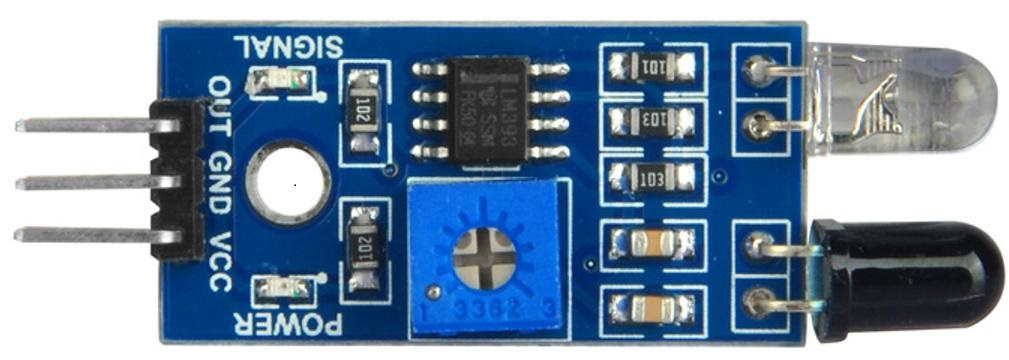
\includegraphics[scale = 0.35]{Media/Figuren/HW-201.jpg}
    \caption{HW-201}
    \label{HW-201}
    \cite{HW-201-hardware} 
\end{figure}
Infrarood sensoren werken door infrarood straling te zenden en te ontvangen. Het zenden gebeurd met een Infrarood led en het ontvangen met een fotodiode. Het is geschikt voor het detecteren van objecten \cite{IR-datasheet}.

In eerste instantie waren HW-201 infrarood sensoren gebruikt voor het detecteren van objecten van 2 tot 30 centimeter. In figuur \ref{HW-201}\cite{HW-201-hardware} is de HW-201 te zien. Voor de eisen van het project is aangegeven dat er vier infrarood sensoren gebruikt moeten worden met in elke hoek één infrarood sensor. De voorste sensoren wijzen naar voren en de achterste sensoren wijzen naar achteren. Door Infra Vroom is er gekozen om vier extra infrarood sensoren te plaatsen, zodat de \gls{Smart-Car} uiteindelijk makkelijker door zijn omgeving kan manoeuvreren. In elke hoek is er één sensor extra geplaatst die naar de zijkant van de \gls{Smart-Car} wijst. Uiteindelijk is ervoor gekozen een ander soort sensor te gebruiken met dezelfde werking, omdat de HW-201 te groot is. De vervangende infrarood sensoren zijn ontworpen door een van de begeleidende docenten en worden alleen voor de \gls{Smart-Car} gebruikt. Deze Infrarood sensoren hebben dezelfde werking als de HW-201 infrarood sensoren alleen is er nu een centrale printplaat in het midden van de \gls{Smart-Car} met in elke hoek een ontvanger, zender en een output pin die op de printplaat kan worden aangesloten. Uiteindelijk is er besloten om de infrarood sensoren te gebruiken om te bepalen of er een blokkade is in de richting waarin de sensor wijst.
\subsubsection{Ultrasonische sensoren}
\begin{figure}[h]
    \centering
    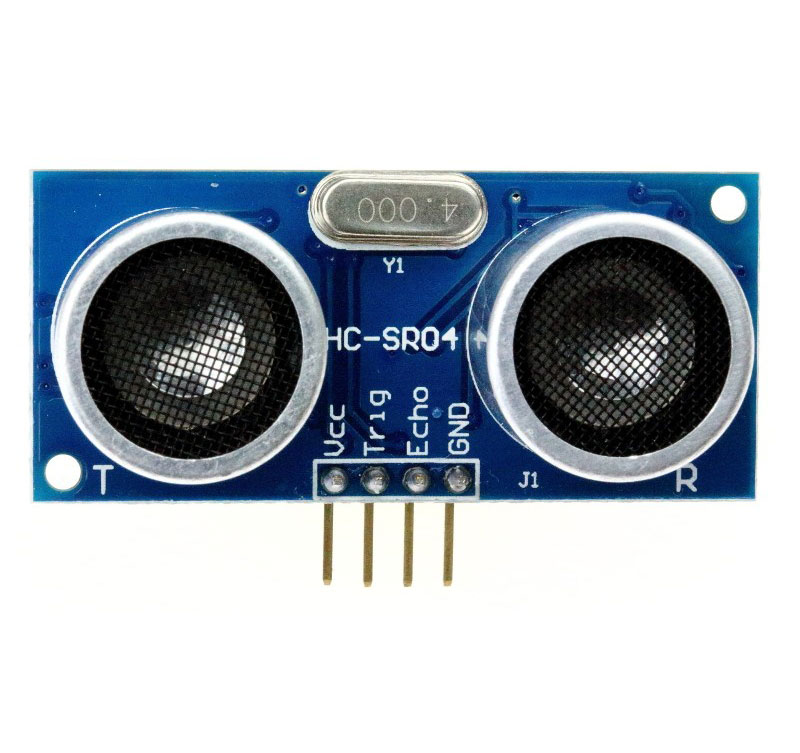
\includegraphics[scale = 0.2]{Media/Figuren/HCSR04-hardware.jpg}
    \caption{HC-SR04}
    \label{HC-SR04-component}
    \cite{HC-SR04-image-RL} 
\end{figure}
Ultrasoon sensoren zenden en ontvangen ultrasoon geluid met een frequentie van 20 kHz en bepaald met behulp van een berekening de afstand tot een object. De HC-SR04 ultrasonische sensor, te zien in figuur \ref{HC-SR04-component}\cite{HC-SR04-image-RL}, is geschikt om afstanden te meten van 4 cm tot 4 m door het gebruik van twee \gls{transducer}s: zender en ontvanger. De \gls{Smart-Car} moet afstanden kunnen meten tot een bepaald object, waardoor de ultrasonische sensor geschikt is voor de eisen van de opdrachtgever\cite{HC-SR04}.

De \gls{Smart-Car} beschikt over drie ultrasonische sensoren: links, rechts en voor. Door deze plaatsing van de sensoren zou de \gls{Smart-Car} door een omgeving moeten kunnen rijden en daarop kunnen reageren. 

\subsubsection{9 Axis Sensor}
De BNO055\cite{AXIS} is een versnellingsmeter, gyroscoop, magnetometer en oriëntatie die wordt gebruikt om de oriëntatie van de \gls{Smart-Car} in de ruimte te meten. Het kan de oriëntatie van een object meten in de vorm van Euler-hoeken (roll, pitch, yaw) of als quaternion.

De BNO055\cite{AXIS} kan worden aangestuurd via een protocol. Via dit protocol kunnen verschillende configuratieparameters ingesteld worden. Momenteel wordt het alleen nog gebruikt om de \gls{Smart-Car} rechtdoor te laten rijden in de gewenste richting. 
\subsection{Actuatoren}
\subsubsection{Motoren}
Om de \gls{Smart-Car} te laten rijden worden 4 motoren gebruikt. Voor het aansturen van de motoren wordt gebruik gemaakt van een \gls{motorshield}, bestaande uit twee belangrijke componenten: een 74HC595N\cite{shiftregister} \gls{shift-register} en twee L293D\cite{h-brug} \gls{H-brug} motor drivers. Het 74HC595N\cite{shiftregister} \gls{shift-register} is een seriële-in, parallel-out \gls{shift-register} met uitgangslatches, dat 8-bits extra digitale uitgangen creëert zonder extra pinnen op de \gls{microcontroller} te gebruiken. Om gegevens naar de chip te sturen, dient men seriële gegevens in te voeren op de SER-pin en SRCLK pulsen te geven aan de klok-ingang. Bij iedere puls wordt het volgende seriële bit overgezet naar het \gls{register}. Na overdracht van alle 8 bits kan de inhoud van het \gls{register} op de parallelle uitgangen worden gezien. Om de inhoud van het \gls{register} op de parallelle uitgangen te laten verschijnen, moet er een latch-puls gegeven worden, door de RCLK-pin te activeren.

De uitgangslatches van het \gls{shift-register} sturen een positief of negatief signaal naar de twee L293D\cite{h-brug} \gls{H-brug} motor drivers, waarmee de vier motoren worden aangestuurd. Door de L293D\cite{h-brug} in combinatie met een \gls{microcontroller} of andere digitale circuits te gebruiken, kan de richting en snelheid van een DC-motor worden geregeld. Het IC beschikt over vier digitale ingangen (twee voor elke motor), waarmee de motor in de gewenste richting kan worden gestuurd. Om de motor aan en uit te zetten, beschikt de L293D\cite{h-brug} tevens over één Enable-ingang per motor, die kan worden aangesloten op een \gls{PWM}-signaal om de motorsnelheid te regelen.

Het is van groot belang om de stroomsterkte van de motor en de spanning van de voeding goed te controleren en af te stemmen op de specificaties van de L293D\cite{h-brug}. Dit moet, omdat het IC een maximale stroom van 600 mA per kanaal kan leveren en is uitgerust met ingebouwde beveiligingsfuncties, zoals \gls{thermische} uitschakeling en bescherming tegen kortsluiting, wat het veilig en betrouwbaar maakt om te gebruiken in diverse toepassingen.

Om een DC-motor in één richting te laten draaien, moeten de logische waarden op IN1 en IN2 voor motor 1 respectievelijk op HIGH en LOW worden gezet. Wanneer de Enable-ingang van de motor hoog is, wordt de motor ingeschakeld en wanneer deze laag is, wordt de motor uitgeschakeld. Bovendien is er na uitgebreid onderzoek vastgesteld dat de maximale \gls{PWM}-waarde voor de motoren niet hoger dan 220 mag zijn, omdat anders de motoren kunnen doorbranden. Dankzij het gebruik van het \gls{motorshield} met de 74HC595N\cite{shiftregister} \gls{shift-register} en L293D\cite{h-brug} \gls{H-brug} motor driver kunnen de motoren op een gecontroleerde en veilige manier worden aangestuurd.

\subsubsection{Servo}
Er zit momenteel 1 servo op de \gls{Smart-Car}. De servo bevindt zich op de voorkant. Op deze servo is de voorste ultrasoon sensor bevestigd. De servo moet ervoor zorgen dat de ultrasoon sensor meer kan detecteren dan alleen vooruit. Dit zorgt ervoor dat de dode hoek kleiner wordt. Voor deze servo zijn verschillende versies code geschreven, dit vanwege verbeteringen en vanwege onduidelijkheden. 

\begin{lstlisting}
#include <Servo.h>
int servoPin = 10;
Servo servo;
int pos = 0;   

void setup() {
  servo.attach(10);}
void loop() {
  for (pos = 60; pos <= 120; pos += 1) { 
    servo.write(pos);              
    delay(30);}
  delay(30);
  for (pos = 120; pos >= 60; pos -= 1) {
    servo.write(pos);              
    delay(30);}}
\end{lstlisting}

De eerste code was geschreven met een library en de functie delay(). In eerste instantie is de code geschreven, om de servo heen en weer te laten zwaaien in een vloeiende beweging. Dit is gerealiseerd door eerst de library servo.h toe te voegen. vervolgens is een servo object aangemaakt, om de servo aan te kunnen sturen. Er is daarnaast een variabele int “angle” aangemaakt, welke gelijk is gesteld aan 0.  In void setup() is de servo pin gedeclareerd met behulp van de functie servo.attach. 
Dan volgt de void loop(), hierin is doormiddel van twee simpele for-loops de geleidelijke beweging gerealiseerd. Deze for-loops passen de hoek van de servo telkens aan met servo.write. Iedere keer dat de for-loop wordt doorlopen, verandert de hoek met 1 graden. De eerste for-loop vergroot de hoek, zolang deze kleiner of gelijk is aan 120 graden. De tweede for-loop verkleint de hoek, zolang de hoek groter of gelijk is aan 60 graden. In deze versie van de code staan in beide for-loops nog delay functies. Dit is niet ideal, want deze stoppen alle code op de Arduino Mega\cite{ArduinoMEGA} voor de duratie van de functie. 

\begin{lstlisting}
int angle;
int pwm;

void setup() {
  pinMode(10, OUTPUT);}

void loop () {
  for (angle = 60; angle <= 120; angle += 1) {
    servoPulse(10, angle);}
  for (angle = 120; angle >= 60; angle -= 1) {
    servoPulse(10, angle);}}
  
void servoPulse (int servo, int angle) {
  pwm = (angle*11) + 500;      // Convert angle to microseconds
  digitalWrite(servo, HIGH);
  delayMicroseconds(pwm);
  digitalWrite(servo, LOW);
  delay(50);                   // Refresh cycle of servo}
\end{lstlisting}

Nadat de eerste versie geschreven was, werd door een leerling van een ander groepje gezegd dat er geen library gebruikt mocht worden. Vanwege de onzekerheid over de correctheid hiervan, is de code herschreven.  Dit keer zonder library\cite{Aansturen-servo-zonder-library}. In deze versie is de pinaanduiding gedaan met “pinMode()” in plaats van “servo.attach()” en is de simpele functie “servo.write()” vervangen door de functie “servoPulse()”. In de functie “servoPulse()” is een 2e variabele int “pwm” gebruikt. Deze is gebruikt om te bepalen hoe lang de servo moet draaien om de gewenste hoek te krijgen. Hiervoor is de berekening op regel 21 van de code uitgevoerd. Door gebruik te maken van “digitalWrite()” en “delayMicroseconds()” is de servo voor de berekende duur op hoog gezet. 

\begin{lstlisting}
#include <Servo.h>
const int servoPin = 10; 
const int servoMinDegrees = 60; 
const int servoMaxDegrees = 120;
Servo servo1;
int servoPosition = servoMinDegrees;    
int servoInterval = 30; 
int servoDegrees = 1;       
int servoDegreeCounter = servoMaxDegrees;
unsigned long currentMillis = 0;    
unsigned long previousServoMillis = 0; 

void setup() {
  Serial.begin(9600);  
  servo1.write(servoPosition); 
  servo1.attach(servoPin);}

void loop() {
  currentMillis = millis();
  servoSweep();}

void servoSweep() {
    while(currentMillis - previousServoMillis >= servoInterval) {
      previousServoMillis += servoInterval;
      servoPosition = servoPosition + servoDegrees; 
      if ((servoPosition == servoMaxDegrees) || (servoPosition == servoMinDegrees)) {
      servoDegrees = - servoDegrees; 
      servoPosition = servoPosition + servoDegrees;}  
    servo1.write(servoPosition);}}
\end{lstlisting}

De 3e versie van de servo code was geschreven toen duidelijk werd dat alleen voor de motorshield geen library gebruikt mocht worden en dus voor de servo wel. Daarnaast waren de eerste twee versies niet ideaal, vanwege het gebruik van de functie “delay()”. Daarom is de code voor de servo voor een derde keer herschreven, dit keer weer met library en zonder de delay functie\cite{Functie-millis-info}. 
Zoals in de 3e versie van de servo code te zien is, is dit voor elkaar gekregen door de functie “millis()” in combinatie met intervallen te gebruiken. Arduino\cite{ArduinoMEGA} houdt automatisch bij hoe lang de programmacode draait, met de functie millis() wordt deze tijd gegeven in milliseconden. Door de begintijd van een opdracht bij te houden en hier de eindtijd van de vorige opdracht of cyclus van af te trekken, kan de verstreken tijd worden bepaald. In deze versie van de servo-code is dit gedaan met de variabelen 
currentMillis en previousServoMillis. Met behulp van een variabele interval, servoInterval, kan tussen deze verstreken tijd en het interval een voorwaarde worden opgesteld, waarna of zolang iets moet gebeuren. Er is in deze versie zo een voorwaarde opgesteld en gebruikt in een while-loop, om iedere keer de servo met 1 graden te laten draaien. Wederom is dit nog de geleidelijke beweging van de servo.
Dit werkte prima als losse code, bij het combineren van de code werkte het echter niet meer. Dit zal in de toekomst dus nog verbeterd en / of aangepast moeten worden. Hierop wordt dieper ingegaan bij “Aanbevelingen”.


\subsection{Matrix}
Achterin de \gls{Smart-Car}, in het midden, bevindt zich een 8x8 matrixbord met 64 LED-punten. Het doel hiervan is om tijdens het rijden een pijl te laten zien op het matrixbord, die de richting aangeeft waarin de \gls{Smart-Car} zich beweegt. Om het bord aan te sluiten, zijn er vijf pinnen: Vcc, GND, DIN, CS en CLK. Vcc is de voedingsingang (+5V), GND geeft de grond aan (-), bij DIN wordt het signaal doorgegeven via het schuifregister en verschijnt op DOUT 16,5 klokcycli later, CS betekent dat de gegevens worden vergrendeld in de cijfer- of besturingsregisters en CLK geeft aan wanneer het leest bij elk opgaand blok signaal. Deze drie pinnen worden gecombineerd met behulp van de LedControl-library.

Gebaseerd op het doel van de codeconstructie, bestaat de code uit 10 hexadecimale combinaties, elk met een volledige richtingpijl. Deze 10 pijlen worden gedeclareerd in een reeks van sizeof en geformuleerd in een void functie. Vervolgens moet voor elke pijl, per richting,individueel worden aangegeven wanneer deze tevoorschijn moet komen. Dit kan eenvoudig worden gedaan door bij het volledige programma de gewenste pijl te selecteren met de aanroep "displayImage(IMAGES[]);". Het resultaat is een kort en efficiënt code-ontwerp dat gemakkelijk aan elk programma kan worden toegevoegd.
Dit proces is tot stand gekomen met behulp van drie codes: 
\begin{enumerate}
    \item Voorbeeldcode: dit is een replica-code die van internet is gehaald om te testen of het scherm goed werkt en om een idee te krijgen voor de eigen code.
    \begin{lstlisting}
#include <MAX7219.h>
int DIN = 50;
int CS =  53;
int CLK = 51;
MAX7219 Matrix(1, DIN, CLK, CS);

// binary represention of a heart shape
const static byte HEART[8] = {
  0b01100110,
  0b10011001,
  0b10000001,
  0b10000001,
  0b01000010,
  0b00100100,
  0b00011000,
  0b00000000};

// The Letter "R"
// human-readable binary representation from left-to-right and top-to-bottom
const static byte R[8] = {
  0b00000000,
  0b01111100,
  0b01000110,
  0b01111100,
  0b01001000,
  0b01000100,
  0b01000010,
  0b00000000};

void setup() {}

void loop() {  
  // First LED in upper left Corner
  Matrix.setLed(1, 0, 0, true);
  delay(1000);
  Matrix.setLed(1, 0, 0, false);
  delay(1000);
  // Make Hearshape from array
  for(int row = 0; row <= 7; row++) {
    Matrix.setRow(1, row, HEART[row]);
    delay(100);}
  delay(1000);
  // Change Intensity to make it pulse
  for(int repeats = 0; repeats < 3; repeats++) {
    // increase intensity
    for(int i = 1; i <= 15; i++) {
      Matrix.setIntensity(1, i);
      delay(20);}
    // decrease intensity
    for(int j = 15; j >= 1; j--) {
      Matrix.setIntensity(1, j);
      delay(20);}}
  delay(1000);
  // Make Letter "R" from array
  for(int row = 0; row <= 7; row++) {
    Matrix.setRow(1, row, R[row]);
    delay(100);}
  delay(1000);
  // invert display
  Matrix.invertDisplay(1);
  delay(1000);  
  // clear display
  Matrix.clearDisplay(1);
  delay(1000);}
    \end{lstlisting}
    \item 1e code: In het eerste ontwerp van de code worden de leds aangestuurd met behulp van een binaire combinatie van getallen. Deze binaire combinatie wordt vervolgens gecombineerd met een array in een void functie. Met deze code-structuur is het gemakkelijk om de pijl op het scherm weer te geven in de actuele rijrichting van de \gls{Smart-Car}. 
    \begin{lstlisting}
void setup() {}

void loop() { 
  up();
  // letterL();}
void up() {
currentMillis = millis();  
while (currentMillis - previousMillis >= matrixdelay) {
  // Make arrowup from array
  for(int row = 0; row <= 7; row++) {
    LedControl(1, row, uparrow[row]);}  
  previousMillis += matrixdelay; //previousMillis = previousMillis + matrixdelay}}
    \end{lstlisting}
    \item Eindproduct: Omdat er 22 verschillende oriëntatie richtingen zijn, zou de combinatie van getallen in binaire vorm, het programma te lang en te complex maken. Als oplossing  is dit programma compacter gemaakt door Hexadecimale waarden te gebruiken die hetzelfde resultaat geven.
    \begin{lstlisting}
#include <LedControl.h>
const int DIN_PIN = 50;
const int CS_PIN = 53;
const int CLK_PIN = 51;

const uint64_t IMAGES[] = {
  0x081c3e0808080808,
  0x08080808083e1c08,
  0x002060ff60200000,
  0x000406ff06040000,
  0x000042e242423c00,
  0x0000424742423c00,
  0x0102040890e0e0f0,
  0x804020100907070f,
  0x0f07070910204080,
  0xf0e0e09008040201};
const int IMAGES_LEN = sizeof(IMAGES)/8;
LedControl display = LedControl(DIN_PIN, CLK_PIN, CS_PIN);

void setup() {
  display.clearDisplay(0);
  display.shutdown(0, false);
  display.setIntensity(0, 5);}

void displayImage(uint64_t image) {
  for (int i = 0; i < 8; i++) {
    byte row = (image >> i * 8) & 0xFF;
    for (int j = 0; j < 8; j++) {
      display.setLed(0, i, j, bitRead(row, j));}
    
void loop() {
  displayImage(IMAGES[i]);}
    \end{lstlisting}
\end{enumerate}
\vspace{80mm} %5mm vertical space #Dit is gedaan zodat de bluetooth afbeelding goed geplaatst wordt
\subsection{Modules}
\subsubsection{Bluetooth}\begin{figure}[h]
    \centering
    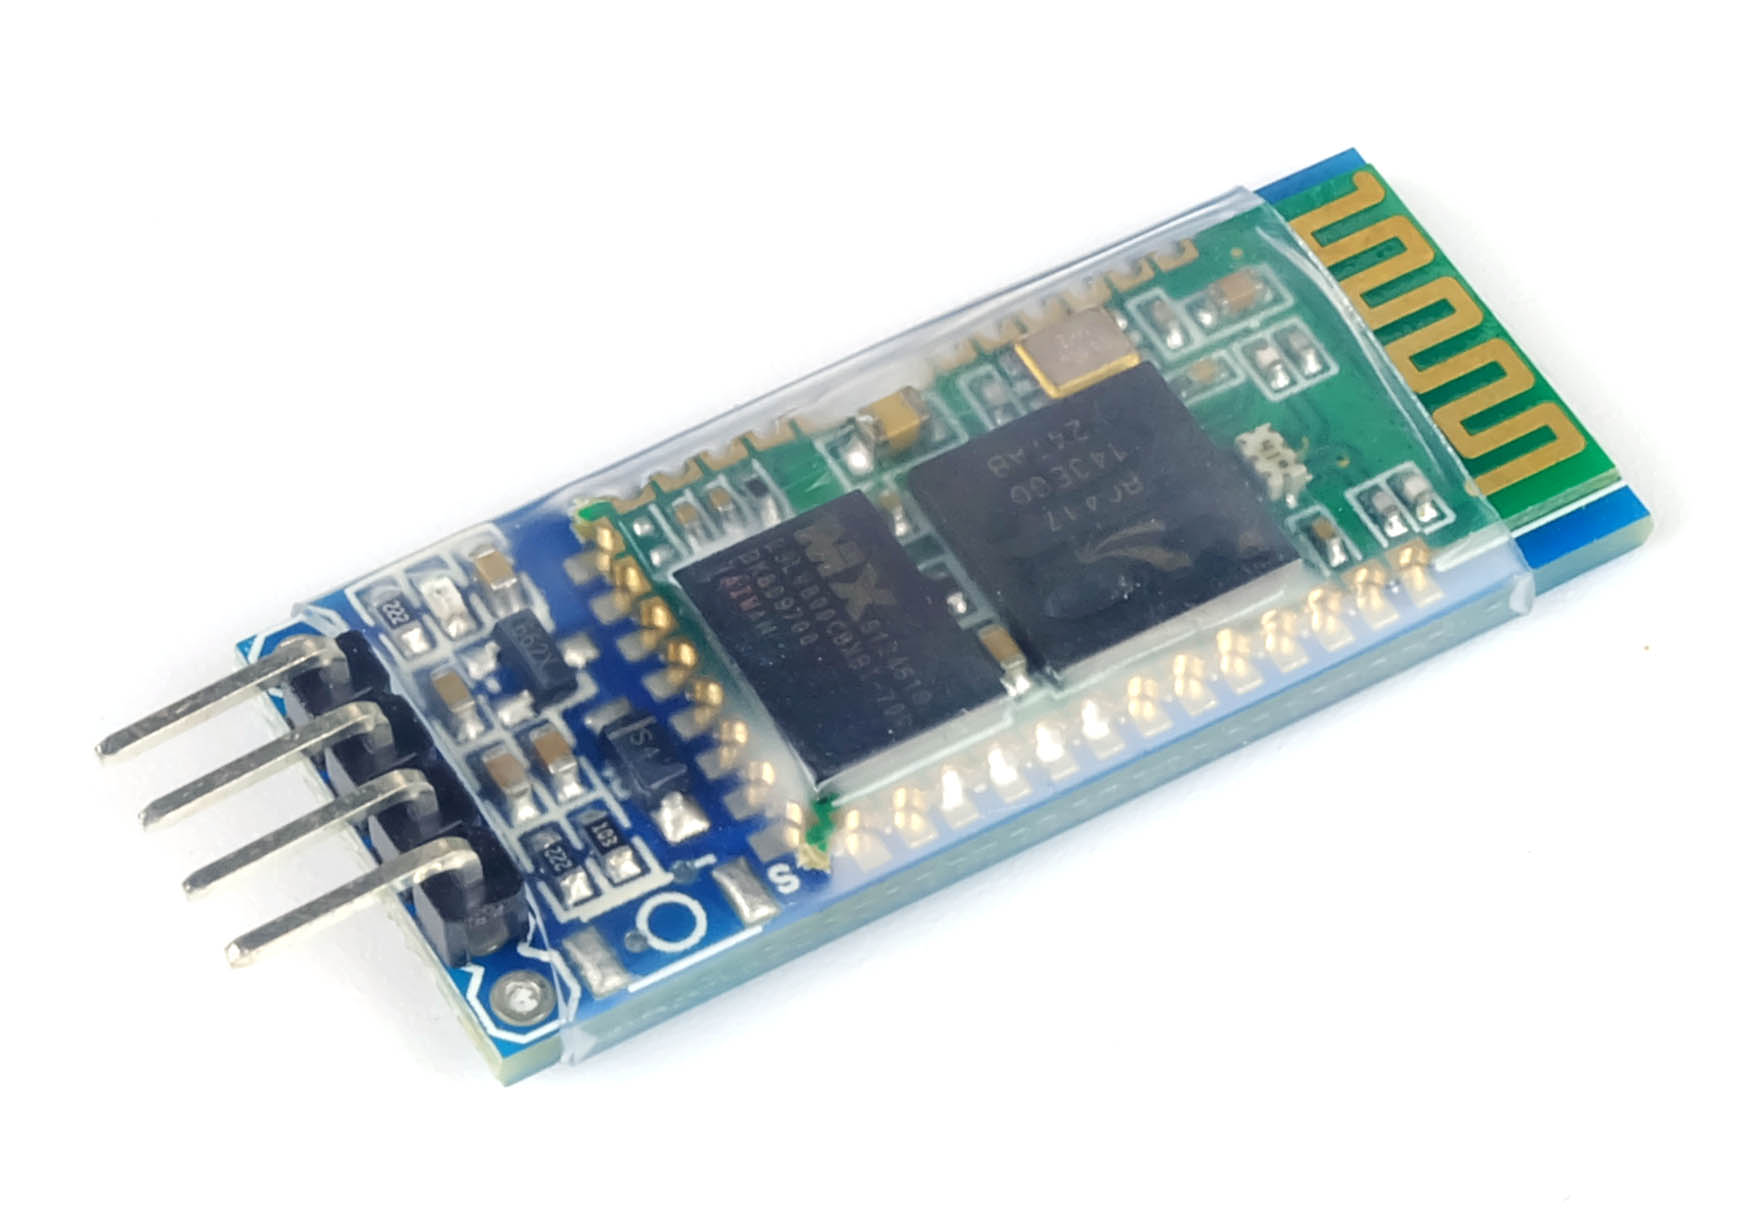
\includegraphics[scale = 0.08]{Media/Figuren/HC-05_hardware.jpg}
    \caption{HC-05}
    \label{HC-05}
    \cite{HC-05-image-fysiek-RL} 
\end{figure}

De HC-05\gls{Bluetooth} module, te zien in figuur \ref{HC-05}\cite{HC-05-image-fysiek-RL}, wordt gebruikt voor het besturen van de \gls{Smart-Car} over een afstand van maximaal 10m. Hierbij is een applicatie gebruikt op de telefoon die door de opdrachtgever is gegeven. Het is de bedoeling dat de \gls{Smart-Car} bepaalde richtingen op kan, welke in het Programma van eisen beschreven staan. 
\subsubsection{Controller}
Tijdens de ontwikkeling van de \gls{Smart-Car} is er een controller ontworpen om een \gls{Smart-Car} aan te sturen met behulp van \gls{RF433MHZ}-chips. Verschillende componenten werden hiervoor gebruikt, waaronder een \gls{TFT-display} met een \gls{ili9341}\cite{ILI3941} IC, twee KY-023 joysticks en een ESP32\cite{ESP32} D1 MINI \gls{microcontroller}.

De ESP32\cite{ESP32} D1 MINI \gls{microcontroller} is een krachtige \gls{microcontroller} die in staat is om draadloze verbindingen te maken en complexe taken uit te voeren. Met de dubbele kern en 240 MHz rekenkracht was de ESP32\cite{ESP32} bij uitstek geschikt voor het verwerken van de gegevens van de twee KY-023 joysticks. De ingebouwde WiFi- en \gls{Bluetooth}-functionaliteit maakte het bovendien mogelijk om draadloos verbinding te maken met andere apparaten, wat tijdens de ontwikkeling van het project handig is.

Het \gls{TFT-display} met de \gls{ili9341}\cite{ILI3941} IC zorgde voor een snelle en efficiënte verwerking van de grafische weergave op het scherm. Dit gaf de mogelijkheid tot snelle en vloeiende weergave van informatie die nodig was om\gls{Smart-Car} te besturen.

De twee KY-023\cite{KY023} joysticks waren aangesloten op de ESP32\cite{ESP32} D1 MINI en na het uitlezen van de waarden, werden deze gekalibreerd en omgezet in een serieel formaat dat verzonden kon worden via de \gls{RF433MHZ}-transceiver. De combinatie van \gls{RF433MHZ} en de joysticks zorgde voor een betrouwbare en responsieve verbinding tussen de controller en de \gls{Smart-Car}, waardoor de \gls{Smart-Car} met precisie bestuurd kon worden in elke richting.

Over het algemeen waren het \gls{TFT-display} met de \gls{ili9341}\cite{ILI3941} IC en de krachtige ESP32\cite{ESP32} D1 MINI \gls{microcontroller} cruciale componenten in het ontwerp van de controller. Deze zorgden namelijk voor een vloeiende en responsieve gebruikerservaring en boden de flexibiliteit en rekenkracht die nodig was om de \gls{Smart-Car} nauwkeurig te kunnen besturen.

Daarnaast is het gebruik van de KY-023\cite{KY023} joysticks, ook een cruciaal component in het ontwerp van onze controller. De joysticks maakten het mogelijk om de \gls{Smart-Car} in elke richting te bewegen en te sturen, waardoor de controle over de \gls{Smart-Car} zeer nauwkeurig was. Dankzij de combinatie van \gls{RF433MHZ} en de joysticks kon de \gls{Smart-Car} met precisie bestuurd worden. Daarnaast zorgde de betrouwbare en responsieve verbinding tussen de controller en de \gls{Smart-Car} voor een vloeiende gebruikerservaring.

\subsection{Behuizing}
De behuizing die alles bij elkaar houdt, bestaat uit vier onderdelen:
\begin{enumerate}
\item De onderkant, een plaat, waarop de motoren en wielen met bouten en moeren zijn bevestigd.\item De boven plaat, waarop de Arduino Mega, servo en alle sensoren zijn gemonteerd.
\item De rechter zijplaat, waarop de rechter ultrasoon sensor bevestigd is.
\item De linker zijplaat, waaraan de linker ultrasoon sensor is vastgemaakt.
\end{enumerate}
De onderdelen zijn gemaakt met behulp van een 3D-printer en het materiaal PLA (Polylactic Acid). Dit is een duurzaam materiaal dat bij verhitting zacht wordt en bij afkoelen een stevig hard vorm behoudt. Dit is eenverschil ten opzichte van traditionele plastics, in dat het harder en steviger is. Om de onderdelen aan elkaar te bevestigen, zijn spacers en schroeven gebruikt, die de onderplaat en bovenplaat aan elkaar vastgeschroefd houden. De rechter en linker zijplaten zijn met schroeven aan de boven plaat gemonteerd. Deze zorgen voor een stevigeconstructie.

\section{Hoe zijn de tussenproducten getest?}
In dit gedeelte wordt het testen van tussenproducten besproken, waaronder infrarood\cite{IR-datasheet}-, ultrasone- en 9-assige\cite{AXIS} sensoren. Om infraroodsensoren\cite{IR-datasheet} te testen, moeten ze worden aangesloten op het \gls{motorshield} en moet de digitale pin op de Arduino Mega 2560\cite{ArduinoMEGA} worden gedefinieerd als de invoerpin. Tijdens het testen werd ontdekt dat twee sensoren waren doorgebrand en vervangen moesten worden. Ultrasone sensoren worden getest door de VCC- en GND-pinnen aan te sluiten op het \gls{motorshield}, en de trigger- en echo-pinnen op een digitale pin op de Arduino Mega 2560\cite{ArduinoMEGA}. De echo-pin wordt gebruikt om de afstand te bepalen door de tijd te meten die nodig is voor het ultrasone geluid om terug te kaatsen. De motordriver\cite{h-brug} wordt aangestuurd door de shiftregister\cite{shiftregister}, die beide op het \gls{motorshield} zijn geplaatst. De shiftregister\cite{shiftregister} decodeert een 8-bits signaal. Hiervoor is een Excel-script geschreven.
\subsection{Sensoren}
Dit hoofdstuk beschrijft hoe infrarood, ultrasonisch en 9-axis sensoren zijn getest.
\subsubsection{Infrarood sensoren}
\begin{figure}[h]
    \centering
    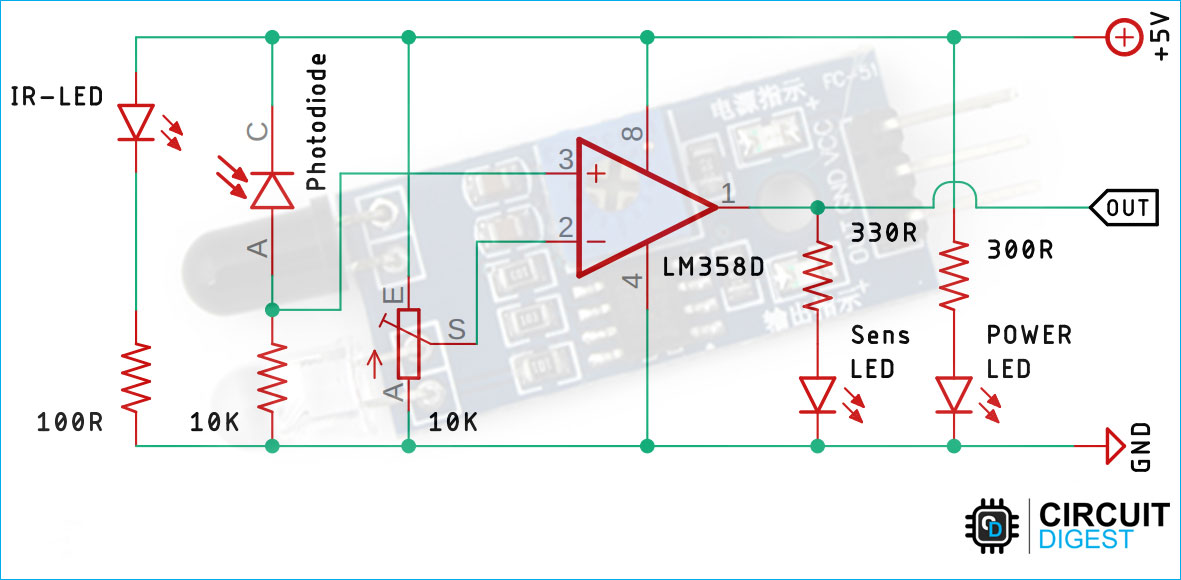
\includegraphics[scale = 0.3]{Media/Figuren/Arduino-IR-Sensor-Circuit.jpg}
    \caption{HW-201 schematische tekening}
    \cite{HW-201-schema}
    \label{schematic-HW-201}   
    \end{figure}
De infrarood sensor beschikt over drie aansluitingen: VCC, GND en een output pin. De VCC wordt op de 5V aangesloten en de GND pin wordt aangesloten op de grond. Beide pinnen worden aangesloten op de motorshield. De output pin word aangesloten op een willekeurige digitale pin op de Arduino Mega 2560. Voor het inlezen van de infrarood sensor moet op de Arduino mega 2560 de digitale pin worden gedefinieerd als input pin. Later kan met de data iets worden gedaan om objecten te vermijden.

De infrarood sensor beschikt over een LM358 IC\cite{LM358-datasheet}. In figuur \eqref{schematic-HW-201}\cite{HW-201-schema} is de schematische tekening te zien van de infrarood sensor. De LM358 vergelijkt twee spanningen op pin 2 en 3, te zien in figuur \eqref{schematic-HW-201}. Afhankelijk van de sterkte van de infrarood straling, komt er een spanning op pin 3 te staan door de fotodiode. Pin 2 is aangesloten op een variabele weerstand. Door aan de variabele weerstand te draaien komt er een andere spanning te staan op pin 2, waarmee de gevoeligheid kan worden ingesteld. Als op pin 3 een hogere spanning komt te staan dan op pin 2, wordt er op pin 1, de output pin, een hoog signaal gegeven. Een laag signaal wordt gegeven als de spanning op pin 3 lager is dan op pin 2.

De infrarood sensor geeft een digitaal signaal op de output pin: 0V of 5V. Voor het meten van de sensoren is gebruik gemaakt van de Seriële monitor in de Arduino IDE met een baudrate van 115200. 

Tijdens het testen werkte twee sensoren niet. Daarvoor zijn er op de oscilloscoop metingen gedaan. Hieruit werd duidelijk dat de sensoren geen 5V genereerden, maar een onbetrouwbare spanning van 2,5V tot 3,5V. In het ideale geval moet er een spanning van 5V op de output pin staan. Hierna is geconcludeerd dat de sensoren opgeblazen waren, waarna er vervolgens nieuwe infrarood sensoren zijn aangevraagd bij  Ad van den Bergh.

Onder deze alinea bevindt zich de code voor het inlezen van de infrarood sensor. In regel 2 en 3 worden de pinnen van de infrarood sensoren gedefinieerd en wordt het aantal infrarood sensoren opgeslagen om later de data eenvoudig uit te lezen en op te slaan. Vervolgens worden er in regel 5-13 een structure gedefineerd voor de infrarood en ultrasonische sensoren. Voor de infrarood sensor wordt de data voor location[5], state, anglepolarity en sensor\_type[30] respectievelijk locatie, status, hoekpositie en het type sensor gebruikt. Daarna wordt in regel 16-25 een structure aangemaakt met de  meegegeven data. In regel 27-30 is een functie IRstate() aangemaakt voor het uitlezen van de sensorwaardes, waarna de waardes in de structure IR\_sensor worden opgeslagen. Daarna worden in regel 33-35 de infrarood sensoren als input gedefinieerd. Ten slotte kan in regel 38 de functie IRstate() worden aangeroepen.


\begin{lstlisting}
//IR SENSOR
uint8_t IR_pins[] = {2, 3, 4, 5, 6, 7, 8, 9};
uint8_t IR_sensoramount = sizeof(IR_pins) / sizeof(IR_pins[0]);

//Struct data localisation
struct data{
  char location[5];
  int state; //IR
  long duration; //US
  int distance; //US
  int angle; //US
  int anglepolarity; //0 = min, 1 = plus, used for IR
  char sensor_type[30];};

struct data IR_sensor[] ={
{"RF", 0, 0, 0, 0, 1, "IR Sensor"},
{"LF", 0, 0, 0, 0, 0, "IR Sensor"},
{"LB", 0, 0, 0, 0, 1, "IR Sensor"},
{"RB", 0, 0, 0, 0, 0, "IR Sensor"},
{"RF", 0, 0, 0, 45, 1, "IR Sensor"},
{"LF", 0, 0, 0, 45, 0, "IR Sensor"},
{"LB", 0, 0, 0, 45, 1, "IR Sensor"},
{"RB", 0, 0, 0, 45, 0, "IR Sensor"}};

void IRstate() { //Reading IR state
  for (int i = 0; i<IR_sensoramount; i++){
    IR_sensor[i].state = digitalRead(IR_pins[i]);}}
   
   void setup() {
   for (int i = 0; i<IR_sensoramount; i++){
    pinMode(IR_pins[i], INPUT);}}
  
  void loop() {
  IRstate();}
\end{lstlisting}
\subsubsection{Ultrasonische sensoren}
De HC-SR04 sensor beschikt over vier pinnen: VCC, GND, trigger en echo. VCC en GND worden op de motorshield voeding aangesloten respectievelijk 5V en grond. De trigger- en echopin wordt aangesloten op een digitale pin van de Arduino mega 2560\cite{HC-SR04}.

De triggerpin is bedoeld om een ultrasonische geluid in de ruimte te sturen door deze pin voor 10 µs hoog te zetten. Nadat de triggerpin laag wordt gezet, wordt de echopin hoog en wacht deze op het ontvangen van het ultrasonisch geluid. Op dit moment wordt de tijd bijgehouden tot het geluid wordt ontvangen. Wanneer er een ultrasonisch geluid wordt ontvangen, wordt de echopin laag. Hieruit kan een afstand worden bepaald, namelijk afstand = snelheid geluid x tijd. Doordat het enige tijd duurt voordat een afstand wordt gemeten, kan een vertraging in de code ontstaan, alhoewel deze miniem zal zijn.

Voor het meten van afstanden van de ultrasonische sensoren is de Seriële monitor  in de Arduino IDE gebruikt met een baudrate van 115200, wat geschikt is voor weergeven van  een afstand tot een object.

Onder deze alinea bevindt zich de code voor het uitlezen en opslaan van de ultrasonische sensor. In regel 2-4 worden de trigger- en echopinnen gedefinieerd, waarbij ook het aantal ultrasoniche sensoren wordt opgeslagen om later eenvoudig de data uit te lezen en op te slaan. Vervolgens wordt in regel 6-14 de structure gedefinieerd voor de infrarood en ultrasonische sensoren. Voor de ultrasonische sensor wordt de data location[5], duration, distance en sensor\_type[30] respectievelijk locatie, duur, afstand en het type sensor gebruikt. Daarna wordt een structure aangemaakt met de meegegeven data. In de regel 22-31 wordt de afstand berekent, waarna het in de structure Sonar\_sensor wordt opgeslagen. Vervolgens worden in regel 33-37 de trigger- en echopin respectievelijk als output en input gedefinieerd. Ten slotte wordt de functie Sonarstate() in regel 39  aangeroepen.
\begin{lstlisting}
//SONAR SENSOR
const int sonartrig_pins[] = {10, 12, 14};
const int sonarecho_pins[] = {11, 13, 15};
int Sonar_sensoramount = sizeof(sonartrig_pins)/sizeof(sonartrig_pins[0]);

//Struct data localisation
struct data{
  char location[5];
  int state; //IR
  long duration; //US
  int distance; //US
  int angle; //US
  int anglepolarity; //0 = min, 1 = plus, used for IR
  char sensor_type[30];};
  
  struct data Sonar_sensor[] ={ //declaring 3 sonar sensors 
  {"FRONT", 0, 0, 0, 0, 0, "Sonar sensor"},
  {"LEFT", 0, 0, 0, 0, "Sonar sensor"},
  {"RIGHT", 0, 0, 0, 0, "Sonar sensor"}};
  
  void Sonarstate(){ //Reading Sonar state/distance
  for (int i = 0; i<Sonar_sensoramount; i++){
  digitalWrite(sonartrig_pins[i], LOW); 
  delayMicroseconds(2);
  digitalWrite(sonartrig_pins[i], HIGH);  //send a pulse
  delayMicroseconds(10);
  digitalWrite(sonartrig_pins[i], LOW); 
  Sonar_sensor[i].duration = pulseIn(sonarecho_pins[i], HIGH);
  Sonar_sensor[i].distance = Sonar_sensor[i].duration * 0.034 / 2;}}
  
void setup() {
for (int i = 0; i<Sonar_sensoramount; i++){
    pinMode(sonarecho_pins[i], INPUT);
    pinMode(sonartrig_pins[i], OUTPUT);}}
  void loop() {
  Sonarstate();}

\end{lstlisting}

\subsection{Actuatoren}
\subsubsection{Motoren}
Motorshield
De motoren worden aangestuurd door een motorshield bestaande uit 3 belangrijke coponenten, 2×L293D\cite{h-brug} en 1×74HC595N\cite{shiftregister}. Deze componenten werken samen volgens het volgende diagram.
\begin{figure}[h]
    \centering
    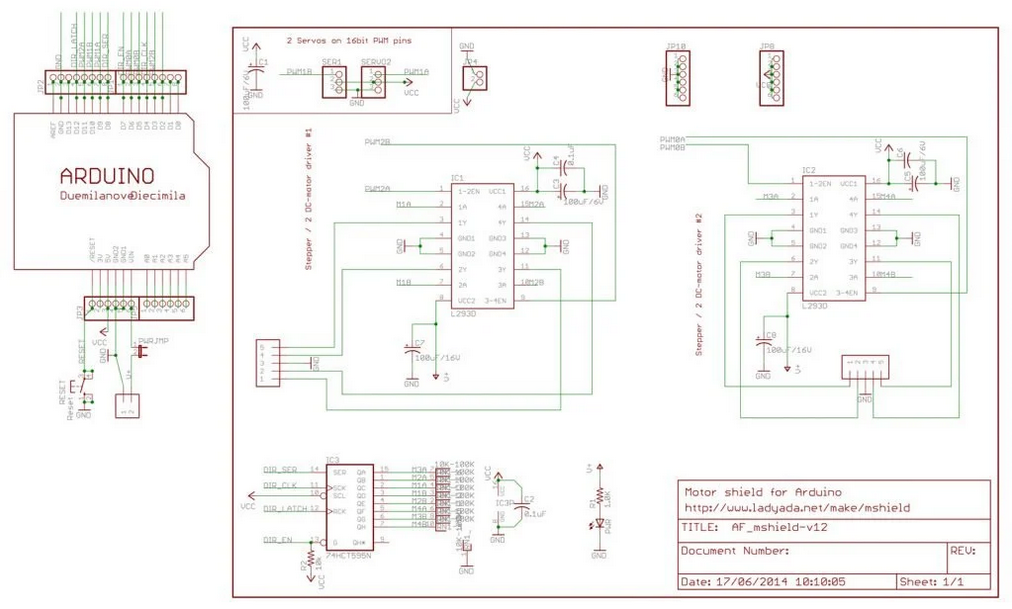
\includegraphics[scale = 0.3]{Media/Figuren/Motorshield_SCHEM.png}
    \caption{Motorshield schematische tekening}
    \label{schematic-Motorshield}   
    \end{figure}

Om het maximale stroomverbruik per kanaal van de H-bruggen te waarborgen, is het totale stroomverbruik per spanning gemeten en zijn vervolgens de resultaten geplot in figuur \ref{Stroomverbruik}. Uit de analyse van de gegevens blijkt dat de motoren niet meer stroom verbruiken dan wat de H-bruggen kunnen verwerken, namelijk 600mA per kanaal. Deze bevindingen zijn van belang omdat ze aangeven dat de H-bruggen veilig en binnen hun capaciteit worden gebruikt in de toepassing van het project.

\begin{figure}[h]
    \centering
    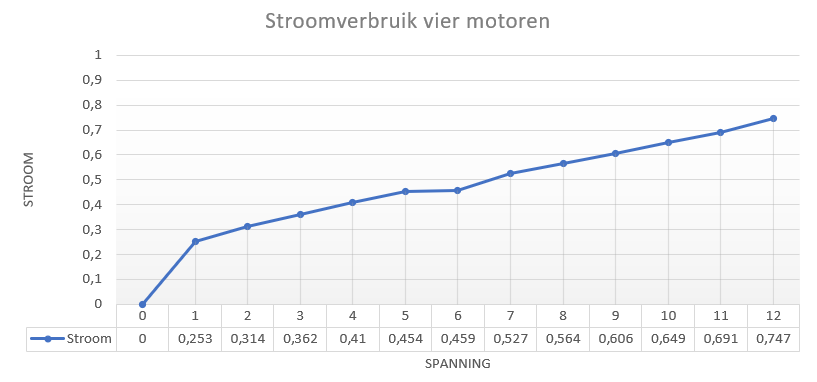
\includegraphics[scale = 0.7]{Media/Figuren/Stroomverbruik.PNG}
    \caption{Stroomverbruik}
    \label{Stroomverbruik}
\end{figure}

\subsubsection{74HC595N Shift Register}
74HC595N\cite{shiftregister} Shift register
De 74HC595N shift register\cite{shiftregister} is een \gls{IC} (Integrated Circuit) dat gebruikt wordt voor het seriele parallelle datatransport. Het IC heeft acht parallelle uitgangen en één seriele ingang. 

Het \gls{IC} heeft 5 ingangen. Het is belangrijk om deze op de juiste momenten aan te sturen, hiervoor heeft Texas Instrument in hun datasheet\cite{shiftregister} een timings \eqref{Timing-register} diagram gemaakt. Hieruit zijn de pinnen makkelijker te ontcijferen en hebben vershillende verschillende pinnen de volgende functies:
\begin{itemize}
    \item Pin 1 (SER): de seriële ingangspen. Hier wordt het seriële signaal dat vanuit de Arduino komt, ingevoerd.
    \item Pin 2 (SRCLK): de shift register klokpen. Hierop wordt een kloksignaal aangesloten dat het verschuiven van de bits in het register triggert.
    \item Pin 3 (RCLK): de latchpen (ook wel register clock genoemd). Hierop wordt een kloksignaal aangesloten dat het overzetten van de inhoud van het shift register naar het output register triggert.
    \item Pin 15 (SRCLR): de shift register clear pen. Hiermee kan het shift register worden gewist.
    \item Pin 16 (OE): de output enable-pen. Hiermee kan de uitgang van het register worden in- of uitgeschakeld.
\end{itemize}
De genoemde ingangen stuur je in de code aan.
\begin{lstlisting}
void MOTOR(int Direction, int MotorPWM1,
int MotorPWM2, int MotorPWM3, int MotorPWM4) {
  SPEED(MotorPWM1, MotorPWM2, MotorPWM3, MotorPWM4);
  digitalWrite(DIR_LATCH, LOW);
  shiftOut(DATA, DIR_CLK, MSBFIRST, Direction);
  digitalWrite(DIR_LATCH, HIGH);}
\end{lstlisting}

\begin{figure} [h]
    \centering
    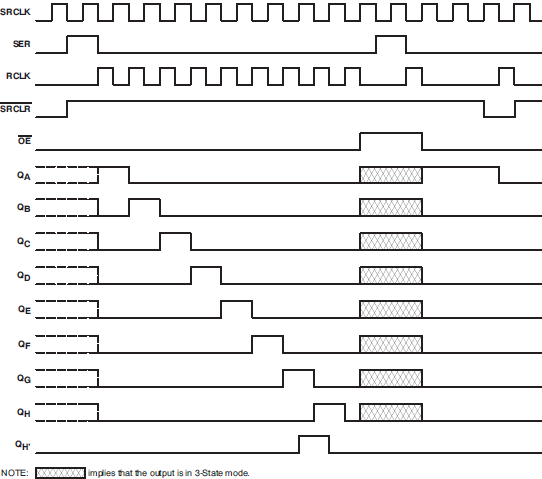
\includegraphics[scale = 0.7]{Media/Figuren/Timing.png}
    \caption{Pin timing \gls{shift-register}}
    \label{Timing-register}   
    \end{figure}
Ook heeft het IC 8 uitgangen, namelijk Q0 t/m Q7, deze zijn verbonden met de L293D. Zie figuur \ref{schematic-Motorshield}.


L293D H-Brug
De L293D\cite{h-brug} is een type H-brug motor driver die de richting en snelheid van DC motoren kan besturen. Het kan tot 600mA aan stroom verwerken en tot twee \gls{DC motoren} tegelijkertijd aansturen. 

De vier ingangspinnen, EN1, EN2, IN1 en IN2, worden gebruikt om de richting en snelheid van de motoren te controleren. 
De uitgangspinnen, OUT1, OUT2, OUT3 en OUT4, zijn verbonden met de motoren. Wanneer de ingangen correct zijn geconfigureerd, kan de L293D\cite{h-brug} de motoren in beide richtingen laten draaien of stoppen. 

De volgende pinnen zijn belangrijk om het IC aan te sturen:
\begin{itemize}
    \item Pin 1, 10 (EN): de enable ingangspinnen. Door een PWM signaal binnen te sturen kan de motorsnelheid aangepast worden.
    \item Pin 11, 6 (IN): de ingangspinnen. Door deze hoog of laag te zetten kan de richting bepaald worden. Deze worden aangestuurd door het \gls{shift-register}\cite{shiftregister}
    \item Pin 2, 5, 9, 12 (OUT): de uitgangspinnen. Deze zijn direct verbonden aan de motoren.
\end{itemize}

\begin{lstlisting}
void SPEED(int MotorPWM1, int MotorPWM2, int MotorPWM3, int MotorPWM4){ 
  analogWrite(PWM2A, MotorPWM1); 
  analogWrite(PWM2B, MotorPWM2);
  analogWrite(PWM0A, MotorPWM3);
  analogWrite(PWM0B, MotorPWM4);}
\end{lstlisting}

Aansturing
Zodra alle datasheets \cite{shiftregister}\cite{h-brug} zijn omgezet in code, kon worden begonnen met het aansturen van de motoren\cite{h-brug}. Gelukkig is de code op een efficiënte manier geschreven, waardoor er functies zijn die op een later moment kunnen worden aangeroepen. 
\begin{lstlisting}
void Forward(){
    MOTOR(DIR_Forward, MotorPWM1, MotorPWM2, MotorPWM3, MotorPWM4);
    displayImage(IMAGES[1]);}
\end{lstlisting}

Om het \gls{motorshield} volledig aan te sturen, is het noodzakelijk om een 8-bits code te verzenden. Deze code is in decimale notatie vastgelegd. Alle beschikbare oriëntatie mogelijkheden zijn opgenomen in tabel 1, figuur \ref{directions}.

\subsubsection{Servo}
Zoals eerder besproken, zijn voor de servo meerdere verschillende versies van de code geschreven. Om te weten of dit werkte moest het getest worden. Het proces van uploaden, uitvoeren, fouten verbeteren en weer herhalen, is het standaard testproces.

Per aanpassing van code werd telkens bepaald wat het verwachtte resultaat was. Vervolgens is de code in een simulator of in de Arduino omgeving geüpload en uitgevoerd. De acties die plaatsvonden zijn vergeleken met het verwachtte resultaat. Werkte dit niet zoals verwacht, dan moest de code worden doorlopen, de fouten worden gelokaliseerd en verbeterd. 

Bij de 1e versie van de servo code ging alles vrij gemakkelijk. Dit was nog een simpele versie, waarbij overigens nog libraries gebruikt waren. Libraries zorgen voor veel simpelere code. Door de functies van de library te gebruiken blijft de code overzichtelijk en zijn de kansen op fouten klein. Bij het testen van deze code is dan ook niet veel fout gegaan. De code werd geüpload naar de Arduino omgeving en uitgevoerd. Hierbij maakte de servo de verwachtte beweging, echter waren de hoeken nog niet naar wens. Dit is toen aangepast waarna het wederom getest werd. 

Voor de 2e versie van de servo code is het standaard proces wederom toegepast. Hierbij moest het proces wel wat vaker herhaald worden om het gewenste resultaat te krijgen, aangezien deze code iets complexer was. 

De 3e versie van de servo code is het meest complex van de drie versies. Hiervoor moest het test proces dan ook vaak herhaald worden. De bedoeling was dat de 3e versie geen delay functies zou bevatten. Om dit voor elkaar te krijgen moest, zoals eerder al uitgelegd, de functie millis() gebruikt worden. Deze functie is aanzienlijk anders dan de eerste twee versies. Na het testproces werkte het echter wel. Toen het in de samengevoegde code werd gezet traden er problemen op. Het resultaat was niet zoals verwacht. De oplossing hiervoor zal nog moeten worden gevonden. 

\subsection{Matrix}
	Voor het testen van het 8x8 Matrix-scherm was de vijf aansluitpinnen pinnen vervolgens schema aangesloten in de arduino bord mega 2560 , en gebruik gemaakt van een replica-code die van het internet hebben gehaald. Replica-code was enkel gebruikt voor testdoeleinden en was niet geïmplementeerd in ons eigen code ontwerp.
\subsection{Modules}
\subsubsection{Bluetooth}
De HC-05 bluetooth module heeft 6 pinnen, waarvan er vier gebruikt worden voor het besturen van de \gls{Smart-Car}. Dit zijn de pinnen: VCC, GND, \gls{Tx en Rx}. VCC en GND worden aangesloten op de voeding van de Arduino Mega 2560, respectievelijk 5V en GND.  De bluetooth Tx pin wordt aangesloten op de Arduino Mega 2560 Rx1 pin. De bluetooth Rx pin werkt op 3,3V en de Arduino Mega 2560 Tx1 pin op 5V. Hiervoor wordt een spanningsdeling geplaatst met een weerstand van 2000\si{\ohm} en 1000\si{\ohm}. De Arduino Rx1 pin wordt aangesloten op bluetooth Tx pin.

Tijdens het testen bleek dat de bluetooth m`odule een hardwarefout had, waardoor de bluetooth module niet wilde verbinden met een apparaat. Zie figuur \eqref{HC-05 fout}. Als oplossing is er een nieuwe module aangevraagd bij de opdrachtgever
\begin{figure}[h]
    \centering
    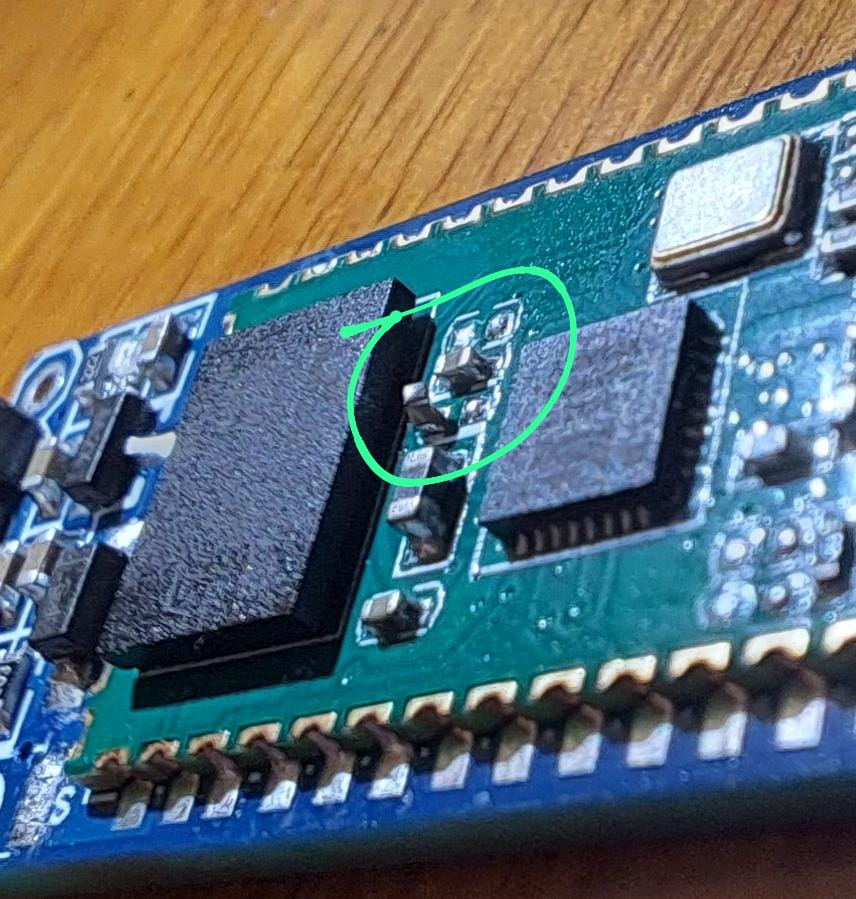
\includegraphics[scale = 0.2]{Media/Figuren/bluetooth hardwarefout.jpg}
    \caption{HC-05 hardwarefout}
    \label{HC-05 fout}
\end{figure}


In de volgende alinea is een eenvoudige code voor het inlezen van bluetooth signalen die vervolgens geprint worden. In het hoofdprogramma worden hier richtingen aan toegekent wat niet wordt weergeven. In regel 5 wordt een variabele aangemaakt die één karakter groot kan zijn. Vervolgens wordt in regel 7-11 de seriële monitor gestart om de richtingen te printen. Daarnaast wordt er een andere seriële monitor gestart waarop de pinnen Tx1 en Rx1 zijn aangesloten, zodat de bluetoothwaarde kan worden uitgelezen. Daarna wordt in regel 15 bekeken of er een waarde is ontvangen door de bluetoothmodule. Als er een waarde is ontvangen, wordt dit in een variabele gezet, te zien in regel 17. Ten slotte wordt in regel 23-43 bij een aantal karakters een taak toegekent.
\newpage
\begin{lstlisting}
char bluetoothValue;
void setup() {//Here the code only runs once.
  Serial.begin(9600);
  Serial1.begin(9600);}

void loop() {
while(Serial1.available()>0){ 
bluetoothValue = Serial1.read();
Serial.print(bluetoothValue);
//Serial.print("\n");
delay(10);
  if(bluetoothValue =='0'){
      Serial.println(" Left ");
  }else if(bluetoothValue == '1'){
      Serial.println(" Forward ");
  }else if(bluetoothValue == '2'){
      Serial.println(" Right ");
  }else if(bluetoothValue == '3'){
      Serial.println(" Backwards ");
  }else if(bluetoothValue == '4'){
      Serial.println(" Faster");
  }else if(bluetoothValue == '5'){
      Serial.println(" Slower");
  }else if(bluetoothValue == '6'){
      Serial.println(" Left rotation");
  }else if(bluetoothValue == '7'){
      Serial.println(" Stop");
  }else if (bluetoothValue == '8'){
      Serial.println(" Right rotation");}}}
\end{lstlisting}
\subsubsection{RF433MHZ}

\subsection{Zelf rijden}
Onze \gls{Smart-Car} is in staat om zelfstandig te rijden, maar momenteel werkt dit nog niet optimaal. De \gls{Smart-Car} zal continu rechtdoor blijven rijden (zoals beschreven in regel 21), totdat niet meer aan een van de voorwaarden wordt voldaan. Tegelijkertijd controleert de \gls{Smart-Car} of er voldoende ruimte is aan de zijkanten; indien dit niet het geval is, zal hij corrigerend optreden.

In regel 4 en daaropvolgende regels worden de variabelen beschreven die de \gls{Smart-Car} nodig heeft om zichzelf rechtuit te laten rijden met behulp van de BNO055\cite{AXIS}, zoals beschreven in regels 23 tot en met 30.

In het geval dat de ultrasone sensoren een foutieve waarde afgeven en de \gls{Smart-Car} niet in staat is om rechtdoor te rijden maar dit toch blijft doen en dus vast komt te zitten, zal dit worden gedetecteerd en zal de \gls{Smart-Car} zichzelf uit deze situatie bevrijden, zoals beschreven in regels 54 en 55.
\begin{lstlisting}
int sidecount = 0;
int rotation = 500;
int driven = 0;
float TargetRoll = 0.0;    
float TargetPitch = 0.0;   
float Tolerance = 1.0;
float MovementThreshold = 0.05;   

void selfdrive(){
imu::Vector<3> accel = bno.getVector(Adafruit_BNO055::VECTOR_ACCELEROMETER);
     MotorPWM1 = 90;
     MotorPWM2 = 90;
     MotorPWM3 = 90;
     MotorPWM4 = 90;
  TargetRoll=AXIS_sensor[0].xaxis;
  float RollError = AXIS_sensor[0].xaxis - TargetRoll;
  float PitchError = AXIS_sensor[0].yaxis - TargetPitch;

  if(Sonar_sensor[0].distance>30 || IR_sensor[2].state==0 || IR_sensor[7].state==0) {
    if (abs(RollError) <= Tolerance && abs(PitchError) <= Tolerance) {
    // Car is driving straight, use default motor PWM values
    MOTOR(DIR_Forward, MotorPWM1, MotorPWM2, MotorPWM3, MotorPWM4);
    displayImage(IMAGES[1]);
  } else {
    // Car is not driving straight, adjust motor PWM values
    displayImage(IMAGES[1]);
    MOTOR(DIR_Forward, MotorPWM1 - RollError, MotorPWM2 + RollError, MotorPWM3 - RollError, MotorPWM4 + RollError);
  }}else if(sidecount==6){
    Backward(); 
    driven = 1;
    delay(750); 
    sidecount = 0;
      if(Sonar_sensor[1].distance>Sonar_sensor[2].distance){
       Left_Rotation();
       delay(rotation);
      }else if(Sonar_sensor[1].distance<Sonar_sensor[2].distance){
        Right_Rotation();
        delay(rotation);
    }}else if(Sonar_sensor[1].distance>Sonar_sensor[2].distance){
    Left_Sideways();
    sidecount++;
  } else if(Sonar_sensor[1].distance<Sonar_sensor[2].distance){
    Right_Sideways();
    sidecount++;
    } else {STOP();}
if(Sonar_sensor[1].distance<10){
  Right_Sideways();}
if(Sonar_sensor[2].distance<10){
  Left_Sideways();}
    if ((abs(accel.x() - AXIS_sensor[0].LOCXAxis) > MovementThreshold || 
      abs(accel.y() - AXIS_sensor[0].LOCYAxis) > MovementThreshold || AXIS_sensor[0].speed <10) && driven==1 ) {
    Backward(); 
    delay(250);
    driven = 0;
    STOP();
    delay(250);
    Right_Rotation();
    delay(rotation);}}
\end{lstlisting}
Om de gemiddelde snelheid van een \gls{Smart-Car} te berekenen, moet de vectoriële som van de acceleratiesnelheden uitgerekend worden.
\begin{equation}
speed = \sqrt{accel.x^2 + accel.y^2}
\end{equation}

\subsection{Excelleren}
\subsubsection{Underglow}
Voor het project \gls{Smart-Car} is een underglow verlichting geïnstalleerd en getest. Hierbij zijn een \gls{WS2812B}\cite{WS2812B} ledstrip en een \gls{ESP8266}\cite{ESP8266} gebruikt. Het doel van de verlichting is om de \gls{Smart-Car} te laten opvallen ten opzichte van andere \gls{Smart-Car}'s en om deze een visueel aantrekkelijke uitstraling te geven. Voor het aansturen van de ledstrip is gebruik gemaakt van de \gls{WLED}-bibliotheek.

\section{Hoe is de documentatie van het proces bijgehouden?}
\subsection{Github}
\subsection{Gezamelijke documenten}
\section{Conclusie}
De hoofdvraag luidde: "Welke stappen zijn er genomen bij het ontwerpen en realiseren van het product voor assessment 1?"
Aan de hand van deelvragen, is hier antwoord op gegeven. 
Zo beschikt de \gls{Smart-Car} van een behuizing met 3 verschillende sensoren. De infrarood sensoren worden gebruikt om te bepalen of er een obstakel in de weg staat, de ultrasoon sensoren worden gebruikt om de afstand tot een object te bepalen, de 9 axis sensor wordt gebruikt om de \gls{Smart-Car} recht te houden. Ook heeft de \gls{Smart-Car} vier motoren om zich mee te verplaatsen en een servo om de dode hoek van de voorste ultrasoon sensor te verkleinen. Verder zit er nog een matrix op de achterkant van de auto die dient om de oriëntatie richting weer te geven. Tenslotte is er ook een \gls{Bluetooth}-module gemonteerd op de auto, waarmee op afstand besturen mogelijk wordt gemaakt. 

Al deze componenten zijn getest door veel onderzoek te doen, uit te proberen of het werkt, fouten verbeteren en herhaal. Alles is zo uitgewerkt tot het één geheel en goed werkende \gls{Smart-Car} vormde. 

 Gedurende dit hele proces is ook een documentatie bijgehouden in Github en in de gezamenlijke Onedrive. 
\section{Aanbevelingen}
Er zijn nog veel dingen te verbeteren aan de \gls{Smart-Car}. 
Aanbevolen wordt daarom, om in de toekomst verder te gaan met het ontwikkelen van de fysieke controller. Daarnaast is het autonome gedeelte van de \gls{Smart-Car} doormiddel van een algoritme gemaakt, die nog erg weinig omvat. Dit kan nog veel beter en verder uitgewerkt worden, onder andere door verdere toepassing van \gls{SLAM} met behulp van de 9 axis sensor. 
\section{Bijlage 1}
\subsection{main.ino}
\begin{lstlisting}
// Library BNO055
#include <Wire.h>
#include <Adafruit_Sensor.h>
#include <Adafruit_BNO055.h>
#include <utility/imumaths.h>
#include <Servo.h>
#include "LedControl.h"

//Header Files
#include "sensor_struct.h"	
#include "pin.h"
#include "directions.h"
#include "readsensor.h"
#include "debug.h"
#include "servo_function.h"
#include "BTread.h"
#include "selfdrive.h"

const int servoPin = 10; // the pin number for the servo signal
const int AngleFRONT = 90; //Set Angle
Servo myservo;

void setup() {
  //Display controll 
  display.clearDisplay(0);
  display.shutdown(0,false);
  display.setIntensity(0, 5); 
  //Servo Write
  myservo.attach(servoPin);
  myservo.write(AngleFRONT);
  //Open Serial Monitor
  Serial.begin(115200); //Serial MON
  Serial.println("Serial Working"); //Serial MON check
  Serial1.begin(9600); //BT serial
  while (!Serial) delay(10); //Wait until serial MON opened
  // bno.setMode(Adafruit_BNO055::OPERATION_MODE_NDOF);
  if(!bno.begin()){Serial.print("Check wiring BNO055"); while(1);}//Initialise BNO055
  
  //Declaring IRpins
  for (int i = 0; i<IR_sensoramount; i++){pinMode(IR_pins[i], INPUT);}
  for (int i = 0; i<Sonar_sensoramount; i++){pinMode(sonarecho_pins[i], INPUT); pinMode(sonartrig_pins[i], OUTPUT);}

  //Pinouts
  pinMode(DIR_CLK, OUTPUT);
  pinMode(DATA, OUTPUT);
  pinMode(DIR_EN, OUTPUT);
  pinMode(DIR_LATCH, OUTPUT);
  pinMode(PWM0B, OUTPUT); //RB
  pinMode(PWM0A, OUTPUT); //LB
  pinMode(PWM2A, OUTPUT); //LF
  pinMode(PWM2B, OUTPUT); //RF 
  void MOTOR(int Direction, int MotorPWM1, int MotorPWM2, int MotorPWM3, int MotorPWM4);
  delay(1000);}

void loop() {
  // bluetoothRead(); //Reading BT values
  // straight();
  selfdrive();
  IRstate(); //Reading IR state
  AXISstate(); //Reading 9Axis state
  Sonarstate(); //Reading Sonar State
  debug(); // Printing sensor states 115200 baud
  // currentMillis = millis(); servoSweep(currentMillis);}
\end{lstlisting}
\subsection{BTread.h}
\begin{lstlisting}
void bluetoothRead(){
     while(Serial1.available()>0){ 
    bluetoothValue = Serial1.read();
    Serial.print(bluetoothValue);
    delay(10);

 if(bluetoothValue =='0'){
    //  Serial.println(" Left ");
      Left_Sideways();
  }else if(bluetoothValue == '1'){
     // Serial.println(" Forward ");
      Forward();
  }else if(bluetoothValue == '2'){
     // Serial.println(" Right ");
      Right_Sideways();
  }else if(bluetoothValue == '3'){
     // Serial.println(" Backwards ");
      Backward();
  }else if(bluetoothValue == '4'){
      //Serial.println(" Faster");
      MotorPWM1 = 130; //LF
      MotorPWM2 = 150; //RF
      MotorPWM3 = 130; //LB
      MotorPWM4 = 150; //RB
      SPEED(MotorPWM1, MotorPWM2, MotorPWM3, MotorPWM4); // go to directions.h to change
  }else if(bluetoothValue == '5'){
     // Serial.println(" Slower"); 
     MotorPWM1 = 87;
     MotorPWM2 = 90;
     MotorPWM3 = 87;
     MotorPWM4 = 90;
      SPEED(MotorPWM1, MotorPWM2, MotorPWM3, MotorPWM4); //go to directions.h to change
  }else if(bluetoothValue == '6'){ 
      //Serial.println(" Left rotation");
      Left_Rotation();
  }else if(bluetoothValue == '7'){
     // Serial.println(" Stop"); 
      STOP();
  }else if (bluetoothValue == '8'){
     // Serial.println(" Right rotation"); 
      Right_Rotation();
  }else if (bluetoothValue == '9'){
     // Serial.println(" Right rotation"); 
      DEMO();
      bluetoothValue = '7';}}}
\end{lstlisting}
\subsection{debug.h}
\begin{lstlisting}
//print the values from the sensors to the Serial Monitor
void debug(){ 
  Serial.print("SONAR SENSOR:");
  for (int i = 0; i<Sonar_sensoramount; i++){//START SONAR
    Serial.print(" | ");
    Serial.print(Sonar_sensor[i].location);
    Serial.print(" [");
    if(Sonar_sensor[i].anglepolarity==1){Serial.print("+");}
    else {Serial.print("-");}
    Serial.print(Sonar_sensor[i].angle);
    Serial.print("] : ");
    Serial.print(Sonar_sensor[i].distance);}//START IR -STOP SONAR
  Serial.print(" |     IR SENSOR:");
  for (int i = 0; i<IR_sensoramount; i++){
    Serial.print(" | ");
    Serial.print(IR_sensor[i].location);
    Serial.print(" [");
    if(IR_sensor[i].anglepolarity==1){Serial.print("+");}
    else {Serial.print("-");}
    Serial.print(IR_sensor[i].angle);
    Serial.print("] : ");
    Serial.print(IR_sensor[i].state);} //END IR-START AXIS
    Serial.print(" |     AXIS SENSOR: X: ");
    Serial.print(AXIS_sensor[0].xaxis);
    Serial.print(" Y: ");
    Serial.print(AXIS_sensor[0].yaxis);
    Serial.print(" Z: ");
    Serial.print(AXIS_sensor[0].zaxis);
    Serial.print(" SPEED: ");
    Serial.print(AXIS_sensor[0].speed);
    Serial.print(" XPOS: ");
    Serial.print(AXIS_sensor[0].LOCXAxis);
    Serial.print(" YPOS: ");
    Serial.print(AXIS_sensor[0].LOCYAxis);
    Serial.println(" |");}
\end{lstlisting}
\subsection{directions.h}
\begin{lstlisting}
//Matrix Pins
const int DIN_PIN = 38;
const int CS_PIN = 42;
const int CLK_PIN = 40;
//Directions
const int DIR_Forward = 39; 
const int DIR_STOP = 0;
const int DIR_Backward = 216;
const int DIR_Left_Sideways = 106;
const int DIR_Right_Sideways = 149;
const int DIR_Left_AAB = 3;
const int DIR_Right_AAB = 36;
const int DIR_Forward_Left_Diagonally = 34;
const int DIR_Backward_Left_Diagonally = 72;
const int DIR_Forward_Right_Diagonally = 5;
const int DIR_Backward_Right_Diagonally = 144;
const int DIR_Left_Rotation = 139;
const int DIR_Right_Rotation = 116;
const int DIR_Left_Front_Rotation = 10;
const int DIR_Right_Front_Rotation = 20;
const int DIR_Left_Back_Rotation = 96;
const int DIR_Right_Back_Rotation = 129;
const int DIR_drift = 116;
const int DIR_Forward_Right_Back_Drift = 38;
const int DIR_Forward_Left_Back_Drift = 7;
const int DIR_Forward_Right_Front_Drift = 37;
const int DIR_Forward_Left_Front_Drift = 35 ;
const int DIR_Backward_Right_Back_Drift = 152;
const int DIR_Backward_Left_Back_Drift = 88;
const int DIR_Backward_Right_Front_Drift = 200;
const int DIR_Backward_Left_Front_Drift = 208;
//Defining display
LedControl display = LedControl(DIN_PIN, CLK_PIN, CS_PIN);
//Matrix HEX codes
const uint64_t IMAGES[] = {
  0x081c3e0808080808, //Backward
  0x08080808083e1c08, //Forward
  0x002060ff60200000, //RIGHT
  0x000406ff06040000, //Left
  0x000042e242423c00, //RightRot
  0x0000424742423c00, //LeftRot
  0x0102040890e0e0f0, //Right diag FW
  0x804020100907070f, //Left diag FW
  0x0f07070910204080, //Left diag BW
  0xf0e0e09008040201, //Right diag BWs
  0x3c4281ffff81423c, //STOP
  0xffe781dbff99bdff //LOL};
const int IMAGES_LEN = sizeof(IMAGES)/8;
void displayImage(uint64_t image) {
  for (int i = 0; i < 8; i++) {
    byte row = (image >> i * 8) & 0xFF;
    for (int j = 0; j < 8; j++) {
      display.setLed(0, i, j, bitRead(row, j));}}}
//MotorSpeed
int MotorPWM1 = 130; //LF
int MotorPWM2 = 150; //RF
int MotorPWM3 = 130; //LB
int MotorPWM4 = 150; //RB
//Writing speed
void SPEED(int MotorPWM1, int MotorPWM2, int MotorPWM3, int MotorPWM4){
  analogWrite(PWM2A, MotorPWM1);
  analogWrite(PWM2B, MotorPWM2);
  analogWrite(PWM0A, MotorPWM3);
  analogWrite(PWM0B, MotorPWM4);}
//Driving motor
void MOTOR(int Direction, int MotorPWM1, int MotorPWM2, int MotorPWM3, int MotorPWM4) {
  SPEED(MotorPWM1, MotorPWM2, MotorPWM3, MotorPWM4);
  digitalWrite(DIR_LATCH, LOW);
  shiftOut(DATA, DIR_CLK, MSBFIRST, Direction);
  digitalWrite(DIR_LATCH, HIGH);}
//Directions
void Forward(){
MOTOR(DIR_Forward, MotorPWM1, MotorPWM2, MotorPWM3, MotorPWM4);
displayImage(IMAGES[1]);}

void STOP(){
MOTOR(DIR_STOP, MotorPWM1, MotorPWM2, MotorPWM3, MotorPWM4);
displayImage(IMAGES[10]);
delay(100);}

void Backward(){
MOTOR(DIR_Backward, MotorPWM1, MotorPWM2,MotorPWM3, MotorPWM4);
displayImage(IMAGES[0]);}

void Left_Sideways(){
MOTOR(DIR_Left_Sideways, MotorPWM1, MotorPWM2, MotorPWM3, MotorPWM4);
displayImage(IMAGES[3]);}

void Right_Sideways(){
MOTOR(DIR_Right_Sideways, MotorPWM1, MotorPWM2, MotorPWM3, MotorPWM4);
displayImage(IMAGES[2]);}

void Left_AAB(){
MOTOR(DIR_Left_AAB, MotorPWM1, MotorPWM2, MotorPWM3, MotorPWM4);
displayImage(IMAGES[11]);}

void Right_AAB(){
MOTOR(DIR_Right_AAB, MotorPWM1, MotorPWM2, MotorPWM3, MotorPWM4);
displayImage(IMAGES[11]);}

void Forward_Left_Diagonally(){
MOTOR(DIR_Forward_Left_Diagonally, MotorPWM1, MotorPWM2, MotorPWM3, MotorPWM4);
displayImage(IMAGES[7]);}

void Backward_Left_Diagonally(){
MOTOR(DIR_Backward_Left_Diagonally, MotorPWM1, MotorPWM2, MotorPWM3, MotorPWM4);
displayImage(IMAGES[8]);}

void Forward_Right_Diagonally(){
MOTOR(DIR_Forward_Right_Diagonally, MotorPWM1, MotorPWM2, MotorPWM3, MotorPWM4);
displayImage(IMAGES[6]);}

void Backward_Right_Diagonally(){
MOTOR(DIR_Backward_Right_Diagonally, MotorPWM1, MotorPWM2, MotorPWM3, MotorPWM4);
displayImage(IMAGES[9]);}

void Left_Rotation(){
MOTOR(DIR_Left_Rotation, MotorPWM1, MotorPWM2, MotorPWM3, MotorPWM4);
displayImage(IMAGES[11]);}

void Right_Rotation(){
MOTOR(DIR_Right_Rotation, MotorPWM1, MotorPWM2, MotorPWM3, MotorPWM4);
displayImage(IMAGES[11]);}

void Left_Front_Rotation(){
MOTOR(DIR_Left_Front_Rotation, MotorPWM1, MotorPWM2, MotorPWM3, MotorPWM4);
displayImage(IMAGES[11]);}

void Right_Front_Rotation(){
MOTOR(DIR_Right_Front_Rotation, MotorPWM1, MotorPWM2, MotorPWM3, MotorPWM4);
displayImage(IMAGES[11]);}

void Left_Back_Rotation(){
MOTOR(DIR_Left_Back_Rotation, MotorPWM1, MotorPWM2, MotorPWM3, MotorPWM4);
displayImage(IMAGES[11]);}

void Right_Back_Rotation(){
MOTOR(DIR_Left_Back_Rotation, MotorPWM1, MotorPWM2, MotorPWM3, MotorPWM4);
displayImage(IMAGES[11]);}

void Forward_Right_Back_Drift(){
MOTOR(DIR_Forward_Right_Back_Drift, MotorPWM1, MotorPWM2, MotorPWM3, MotorPWM4);
displayImage(IMAGES[11]);}

void Forward_Left_Back_Drift(){
MOTOR(DIR_Forward_Left_Back_Drift, MotorPWM1, MotorPWM2, MotorPWM3, MotorPWM4);
displayImage(IMAGES[11]);}

void Forward_Right_Front_Drift(){
MOTOR(DIR_Forward_Right_Front_Drift, MotorPWM1, MotorPWM2, MotorPWM3, MotorPWM4);
displayImage(IMAGES[11]);}

void Forward_Left_Front_Drift(){
MOTOR(DIR_Forward_Left_Front_Drift, MotorPWM1, MotorPWM2, MotorPWM3, MotorPWM4);
displayImage(IMAGES[11]);}

void Backward_Right_Back_Drift(){
MOTOR(DIR_Backward_Right_Back_Drift, MotorPWM1, MotorPWM2, MotorPWM3, MotorPWM4);
displayImage(IMAGES[11]);}

void Backward_Left_Back_Drift(){
MOTOR(DIR_Backward_Left_Back_Drift, MotorPWM1, MotorPWM2, MotorPWM3, MotorPWM4);
displayImage(IMAGES[11]);}

void Backward_Right_Front_Drift(){
MOTOR(DIR_Backward_Right_Front_Drift, MotorPWM1, MotorPWM2, MotorPWM3, MotorPWM4);
displayImage(IMAGES[11]);}

void Backward_Left_Front_Drift(){
MOTOR(DIR_Backward_Left_Front_Drift, MotorPWM1, MotorPWM2, MotorPWM3, MotorPWM4);
displayImage(IMAGES[11]);}

//Demo scene
void DEMO(){
 Forward();
 delay(2000);
 STOP();
 delay(500);

 Backward();
 delay(2000);
 STOP();
 delay(500);

 Left_Sideways();
 delay(2000);
 STOP();
 delay(500);

 Right_Sideways();
 delay(2000);
 STOP();
 delay(500);

 Left_AAB();
 delay(2000);
 STOP();
 delay(500);

 Right_AAB();
 delay(2000);
 STOP();
 delay(500);

 Forward_Left_Diagonally();
 delay(2000);
 STOP();
 delay(500);

 Backward_Left_Diagonally();
 delay(2000);
 STOP();
 delay(500);

 Forward_Right_Diagonally();
 delay(2000);
 STOP();
 delay(500);

 Backward_Right_Diagonally();
 delay(2000);
 STOP();
 delay(500);


 Left_Rotation();
 delay(2000);
 STOP();
 delay(500);

 Right_Rotation();
 delay(2000);
 STOP();
 delay(500);

 Left_Front_Rotation();
 delay(2000);
 STOP();
 delay(500);

 Right_Front_Rotation();
 delay(2000);
 STOP();
 delay(500);

 Left_Back_Rotation();
 delay(2000);
 STOP();
 delay(500);

 Right_Back_Rotation();
 delay(2000);
 STOP();
 delay(500);

 Forward_Right_Back_Drift();
 delay(2000);
 STOP();
 delay(500);

 Forward_Left_Back_Drift();
 delay(2000);
 STOP();
 delay(500);

 Forward_Right_Front_Drift();
 delay(2000);
 STOP();
 delay(500);
 
 Forward_Left_Front_Drift();
 delay(2000);
 STOP();
 delay(500);

 Backward_Right_Back_Drift();
 delay(2000);
 STOP();
 delay(500);

 Backward_Left_Back_Drift();
 delay(2000);
 STOP();
 delay(500);

 Backward_Right_Front_Drift();
 delay(2000);
 STOP();
 delay(500);

 Backward_Left_Front_Drift();
 delay(2000);
 STOP();
 delay(500);}
\end{lstlisting}
\subsection{pin.h}
\begin{lstlisting}
//Motorshield PMW
const int PWM2A = 11;
const int PWM2B = 3;
const int PWM0A = 6;
const int PWM0B = 5;
//Motorshield data
const int DIR_CLK = 4;
const int DIR_EN = 7;
const int DATA = 8;
const int DIR_LATCH = 12;
//IR SENSOR
const int IR_pins[] = {22, 24, 26, 28, 30, 32, 34, 36};
const int IR_sensoramount = sizeof(IR_pins) / sizeof(IR_pins[0]);
//SONAR SENSOR
const int sonartrig_pins[] = {25, 33, 29};
const int sonarecho_pins[] = {23, 31, 27};
const int Sonar_sensoramount = sizeof(sonartrig_pins) / sizeof(sonartrig_pins[0]);
//9 Axis I2C adress
Adafruit_BNO055 bno = Adafruit_BNO055(-1, 0x28, &Wire);
//BT char
char bluetoothValue;
\end{lstlisting}
\subsection{readsensor.h}
\begin{lstlisting}
/* Set the delay between fresh samples */
#define BNO055_SAMPLERATE_DELAY_MS (100)
void IRstate() { //Reading IR state
  for (int i = 0; i<IR_sensoramount; i++){
    IR_sensor[i].state = digitalRead(IR_pins[i]);}}

void Sonarstate(){ //Reading Sonar state/distance
  for (int i = 0; i<Sonar_sensoramount; i++){
  digitalWrite(sonartrig_pins[i], LOW); 
  delayMicroseconds(2);
  digitalWrite(sonartrig_pins[i], HIGH); // set trigger pin to High to send a pulse into the real world
  delayMicroseconds(10);
  digitalWrite(sonartrig_pins[i], LOW); 
  Sonar_sensor[i].duration = pulseIn(sonarecho_pins[i], HIGH); // measure the time it takes to receive the pulse
  Sonar_sensor[i].distance = Sonar_sensor[i].duration * 0.034 / 2; //calculate the distance in cm}}

void AXISstate(){//Reading 9Axis State
  imu::Vector<3> euler = bno.getVector(Adafruit_BNO055::VECTOR_EULER);
  AXIS_sensor[0].xaxis = euler.x();
  AXIS_sensor[0].yaxis = euler.y();
  AXIS_sensor[0].zaxis = euler.z();
  imu::Vector<3> accel = bno.getVector(Adafruit_BNO055::VECTOR_ACCELEROMETER);
  AXIS_sensor[0].speed = sqrt(pow(accel.x(), 2) + pow(accel.y(), 2) + pow(accel.z(), 2));
  AXIS_sensor[0].LOCXAxis = accel.x();
  AXIS_sensor[0].LOCYAxis = accel.y();
  /* Display the floating point data */
  delay(BNO055_SAMPLERATE_DELAY_MS);}
\end{lstlisting}
\subsection{sensor\_struct.h}
\begin{lstlisting}
//Struct data localisation
struct data{
  char location[5];
  int state; //IR
  long duration; //US
  int distance; //US
  int angle; //US
  int anglepolarity; //0 = min, 1 = plus 
  char sensor_type[30];};

//declaring 8 IR sensors by using a struct
struct data IR_sensor[] ={
  {"LB", 0, 0, 0, 180, 1, "IR Sensor"},
  {"LB", 0, 0, 0, 90, 0, "IR Sensor"},
  {"LF", 0, 0, 0, 0, 1, "IR Sensor"},
  {"LF", 0, 0, 0, 90, 0, "IR Sensor"},
  {"RB", 0, 0, 0, 180, 1, "IR Sensor"},
  {"RB", 0, 0, 0, 90, 1, "IR Sensor"},
  {"RF", 0, 0, 0, 90, 1, "IR Sensor"},
  {"RF", 0, 0, 0, 0, 1, "IR Sensor"}};

//declaring 3 sonar sensors by using a struct
struct data Sonar_sensor[] ={ 
  {"FRONT", 0, 0, 0, 0, 0, "Sonar sensor"},
  {"LEFT", 0, 0, 0, 0, "Sonar sensor"},
  {"RIGHT", 0, 0, 0, 0, "Sonar sensor"}};

//AxisSensor struct
struct axis{
  float xaxis;
  float yaxis;
  float zaxis;
  float speed;
  float LOCXAxis;
  float LOCYAxis;
  char sensor_type[30];};

//AxisSensor data struct
struct axis AXIS_sensor[] ={
  {0, 0, 0, 0, 0, 0, "9 Axis Sensor"}};
\end{lstlisting}
\subsection{selfdrive.h}
\begin{lstlisting}
int sidecount = 0;
int rotation = 500;
int driven = 0;
float TargetRoll = 0.0;    
float TargetPitch = 0.0;   
float Tolerance = 1.0;
float MovementThreshold = 0.05;   

void selfdrive(){
imu::Vector<3> accel = bno.getVector(Adafruit_BNO055::VECTOR_ACCELEROMETER);
     MotorPWM1 = 90;
     MotorPWM2 = 90;
     MotorPWM3 = 90;
     MotorPWM4 = 90;
  TargetRoll=AXIS_sensor[0].xaxis;
  float RollError = AXIS_sensor[0].xaxis - TargetRoll;
  float PitchError = AXIS_sensor[0].yaxis - TargetPitch;

  if(Sonar_sensor[0].distance>30 || IR_sensor[2].state==0 || IR_sensor[7].state==0) {
    if (abs(RollError) <= Tolerance && abs(PitchError) <= Tolerance) {
    // Car is driving straight, use default motor PWM values
    MOTOR(DIR_Forward, MotorPWM1, MotorPWM2, MotorPWM3, MotorPWM4);
    displayImage(IMAGES[1]);
  } else {
    // Car is not driving straight, adjust motor PWM values
    displayImage(IMAGES[1]);
    MOTOR(DIR_Forward, MotorPWM1 - RollError, MotorPWM2 + RollError, MotorPWM3 - RollError, MotorPWM4 + RollError);
  }}else if(sidecount==6){
    Backward(); 
    driven = 1;
    delay(750); 
    sidecount = 0;
      if(Sonar_sensor[1].distance>Sonar_sensor[2].distance){
       Left_Rotation();
       delay(rotation);
      }else if(Sonar_sensor[1].distance<Sonar_sensor[2].distance){
        Right_Rotation();
        delay(rotation);
    }}else if(Sonar_sensor[1].distance>Sonar_sensor[2].distance){
    Left_Sideways();
    sidecount++;
  } else if(Sonar_sensor[1].distance<Sonar_sensor[2].distance){
    Right_Sideways();
    sidecount++;
    } else {STOP();}
if(Sonar_sensor[1].distance<10){
  Right_Sideways();}
if(Sonar_sensor[2].distance<10){
  Left_Sideways();}
    if ((abs(accel.x() - AXIS_sensor[0].LOCXAxis) > MovementThreshold || 
      abs(accel.y() - AXIS_sensor[0].LOCYAxis) > MovementThreshold || AXIS_sensor[0].speed <10) && driven==1 ) {
    Backward(); 
    delay(250);
    driven = 0;
    STOP();
    delay(250);
    Right_Rotation();
    delay(rotation);}}
\end{lstlisting}
\phantomsection
\addcontentsline{toc}{section}{Oriëntatie mogelijkheden}
% Please add the following required packages to your document preamble:
% \usepackage[table,xcdraw]{xcolor}
% If you use beamer only pass "xcolor=table" option, i.e. \documentclass[xcolor=table]{beamer}
\begin{table}[h]
\small
\begin{tabular}{cccllllllll}
\rowcolor[HTML]{4472C4} 
{\color[HTML]{FFFFFF} \textbf{DEC}} & {\color[HTML]{FFFFFF} \textbf{BIN}} & {\color[HTML]{FFFFFF} \textbf{Direction}} & {\color[HTML]{FFFFFF} \textbf{QH}} & {\color[HTML]{FFFFFF} \textbf{QG}} & {\color[HTML]{FFFFFF} \textbf{QF}} & {\color[HTML]{FFFFFF} \textbf{QE}} & {\color[HTML]{FFFFFF} \textbf{QD}} & {\color[HTML]{FFFFFF} \textbf{QC}} & {\color[HTML]{FFFFFF} \textbf{QB}} & {\color[HTML]{FFFFFF} \textbf{QA}} \\ \hline
\multicolumn{3}{|c|}{\textit{\textbf{Standard}}} & \multicolumn{1}{l|}{\cellcolor[HTML]{FFFFFF}M4B} & \multicolumn{1}{l|}{\cellcolor[HTML]{FFFFFF}M3B} & \multicolumn{1}{l|}{\cellcolor[HTML]{FFFFFF}M4A} & \multicolumn{1}{l|}{\cellcolor[HTML]{FFFFFF}M2B} & \multicolumn{1}{l|}{\cellcolor[HTML]{FFFFFF}M1B} & \multicolumn{1}{l|}{\cellcolor[HTML]{FFFFFF}M1A} & \multicolumn{1}{l|}{\cellcolor[HTML]{FFFFFF}M2A} & \multicolumn{1}{l|}{\cellcolor[HTML]{FFFFFF}M3A} \\ \hline
\rowcolor[HTML]{D9E1F2} 
\multicolumn{1}{|c|}{\cellcolor[HTML]{D9E1F2}39} & \multicolumn{1}{c|}{\cellcolor[HTML]{D9E1F2}00100111} & \multicolumn{1}{c|}{\cellcolor[HTML]{D9E1F2}Forward} & \multicolumn{1}{l|}{\cellcolor[HTML]{D9E1F2}0} & \multicolumn{1}{l|}{\cellcolor[HTML]{D9E1F2}0} & \multicolumn{1}{l|}{\cellcolor[HTML]{D9E1F2}1} & \multicolumn{1}{l|}{\cellcolor[HTML]{D9E1F2}0} & \multicolumn{1}{l|}{\cellcolor[HTML]{D9E1F2}0} & \multicolumn{1}{l|}{\cellcolor[HTML]{D9E1F2}1} & \multicolumn{1}{l|}{\cellcolor[HTML]{D9E1F2}1} & \multicolumn{1}{l|}{\cellcolor[HTML]{D9E1F2}1} \\ \hline
\multicolumn{1}{|c|}{216} & \multicolumn{1}{c|}{11011000} & \multicolumn{1}{c|}{Backward} & \multicolumn{1}{l|}{\cellcolor[HTML]{FFFFFF}1} & \multicolumn{1}{l|}{\cellcolor[HTML]{FFFFFF}1} & \multicolumn{1}{l|}{\cellcolor[HTML]{FFFFFF}0} & \multicolumn{1}{l|}{\cellcolor[HTML]{FFFFFF}1} & \multicolumn{1}{l|}{\cellcolor[HTML]{FFFFFF}1} & \multicolumn{1}{l|}{\cellcolor[HTML]{FFFFFF}0} & \multicolumn{1}{l|}{\cellcolor[HTML]{FFFFFF}0} & \multicolumn{1}{l|}{\cellcolor[HTML]{FFFFFF}0} \\ \hline
\rowcolor[HTML]{D9E1F2} 
\multicolumn{1}{|c|}{\cellcolor[HTML]{D9E1F2}0} & \multicolumn{1}{c|}{\cellcolor[HTML]{D9E1F2}00000000} & \multicolumn{1}{c|}{\cellcolor[HTML]{D9E1F2}Stop} & \multicolumn{1}{l|}{\cellcolor[HTML]{D9E1F2}0} & \multicolumn{1}{l|}{\cellcolor[HTML]{D9E1F2}0} & \multicolumn{1}{l|}{\cellcolor[HTML]{D9E1F2}0} & \multicolumn{1}{l|}{\cellcolor[HTML]{D9E1F2}0} & \multicolumn{1}{l|}{\cellcolor[HTML]{D9E1F2}0} & \multicolumn{1}{l|}{\cellcolor[HTML]{D9E1F2}0} & \multicolumn{1}{l|}{\cellcolor[HTML]{D9E1F2}0} & \multicolumn{1}{l|}{\cellcolor[HTML]{D9E1F2}0} \\ \hline
\rowcolor[HTML]{FFFFFF} 
 &  &  & \multicolumn{8}{l}{\cellcolor[HTML]{FFFFFF}} \\ \hline
\multicolumn{11}{|c|}{\textit{\textbf{Directions}}} \\ \hline
\rowcolor[HTML]{D9E1F2} 
\multicolumn{1}{|c|}{\cellcolor[HTML]{D9E1F2}106} & \multicolumn{1}{c|}{\cellcolor[HTML]{D9E1F2}01101010} & \multicolumn{1}{c|}{\cellcolor[HTML]{D9E1F2}Left\_Sideways} & \multicolumn{1}{l|}{\cellcolor[HTML]{D9E1F2}0} & \multicolumn{1}{l|}{\cellcolor[HTML]{D9E1F2}1} & \multicolumn{1}{l|}{\cellcolor[HTML]{D9E1F2}1} & \multicolumn{1}{l|}{\cellcolor[HTML]{D9E1F2}0} & \multicolumn{1}{l|}{\cellcolor[HTML]{D9E1F2}1} & \multicolumn{1}{l|}{\cellcolor[HTML]{D9E1F2}0} & \multicolumn{1}{l|}{\cellcolor[HTML]{D9E1F2}1} & \multicolumn{1}{l|}{\cellcolor[HTML]{D9E1F2}0} \\ \hline
\rowcolor[HTML]{FFFFFF} 
\multicolumn{1}{|c|}{\cellcolor[HTML]{FFFFFF}34} & \multicolumn{1}{c|}{\cellcolor[HTML]{FFFFFF}00100010} & \multicolumn{1}{c|}{\cellcolor[HTML]{FFFFFF}Forward\_Left\_Diagonally} & \multicolumn{1}{l|}{\cellcolor[HTML]{FFFFFF}0} & \multicolumn{1}{l|}{\cellcolor[HTML]{FFFFFF}0} & \multicolumn{1}{l|}{\cellcolor[HTML]{FFFFFF}1} & \multicolumn{1}{l|}{\cellcolor[HTML]{FFFFFF}0} & \multicolumn{1}{l|}{\cellcolor[HTML]{FFFFFF}0} & \multicolumn{1}{l|}{\cellcolor[HTML]{FFFFFF}0} & \multicolumn{1}{l|}{\cellcolor[HTML]{FFFFFF}1} & \multicolumn{1}{l|}{\cellcolor[HTML]{FFFFFF}0} \\ \hline
\rowcolor[HTML]{D9E1F2} 
\multicolumn{1}{|c|}{\cellcolor[HTML]{D9E1F2}72} & \multicolumn{1}{c|}{\cellcolor[HTML]{D9E1F2}01001000} & \multicolumn{1}{c|}{\cellcolor[HTML]{D9E1F2}Backward\_Left\_Diagonally} & \multicolumn{1}{l|}{\cellcolor[HTML]{D9E1F2}0} & \multicolumn{1}{l|}{\cellcolor[HTML]{D9E1F2}1} & \multicolumn{1}{l|}{\cellcolor[HTML]{D9E1F2}0} & \multicolumn{1}{l|}{\cellcolor[HTML]{D9E1F2}0} & \multicolumn{1}{l|}{\cellcolor[HTML]{D9E1F2}1} & \multicolumn{1}{l|}{\cellcolor[HTML]{D9E1F2}0} & \multicolumn{1}{l|}{\cellcolor[HTML]{D9E1F2}0} & \multicolumn{1}{l|}{\cellcolor[HTML]{D9E1F2}0} \\ \hline
\rowcolor[HTML]{FFFFFF} 
\multicolumn{1}{|c|}{\cellcolor[HTML]{FFFFFF}3} & \multicolumn{1}{c|}{\cellcolor[HTML]{FFFFFF}00000011} & \multicolumn{1}{c|}{\cellcolor[HTML]{FFFFFF}Left\_AAB} & \multicolumn{1}{l|}{\cellcolor[HTML]{FFFFFF}0} & \multicolumn{1}{l|}{\cellcolor[HTML]{FFFFFF}0} & \multicolumn{1}{l|}{\cellcolor[HTML]{FFFFFF}0} & \multicolumn{1}{l|}{\cellcolor[HTML]{FFFFFF}0} & \multicolumn{1}{l|}{\cellcolor[HTML]{FFFFFF}0} & \multicolumn{1}{l|}{\cellcolor[HTML]{FFFFFF}0} & \multicolumn{1}{l|}{\cellcolor[HTML]{FFFFFF}1} & \multicolumn{1}{l|}{\cellcolor[HTML]{FFFFFF}1} \\ \hline
\rowcolor[HTML]{D9E1F2} 
\multicolumn{1}{|c|}{\cellcolor[HTML]{D9E1F2}139} & \multicolumn{1}{c|}{\cellcolor[HTML]{D9E1F2}10001011} & \multicolumn{1}{c|}{\cellcolor[HTML]{D9E1F2}Left\_Rotation} & \multicolumn{1}{l|}{\cellcolor[HTML]{D9E1F2}1} & \multicolumn{1}{l|}{\cellcolor[HTML]{D9E1F2}0} & \multicolumn{1}{l|}{\cellcolor[HTML]{D9E1F2}0} & \multicolumn{1}{l|}{\cellcolor[HTML]{D9E1F2}0} & \multicolumn{1}{l|}{\cellcolor[HTML]{D9E1F2}1} & \multicolumn{1}{l|}{\cellcolor[HTML]{D9E1F2}0} & \multicolumn{1}{l|}{\cellcolor[HTML]{D9E1F2}1} & \multicolumn{1}{l|}{\cellcolor[HTML]{D9E1F2}1} \\ \hline
\rowcolor[HTML]{FFFFFF} 
\multicolumn{1}{|c|}{\cellcolor[HTML]{FFFFFF}10} & \multicolumn{1}{c|}{\cellcolor[HTML]{FFFFFF}00001010} & \multicolumn{1}{c|}{\cellcolor[HTML]{FFFFFF}Left\_Front\_Rotation} & \multicolumn{1}{l|}{\cellcolor[HTML]{FFFFFF}0} & \multicolumn{1}{l|}{\cellcolor[HTML]{FFFFFF}0} & \multicolumn{1}{l|}{\cellcolor[HTML]{FFFFFF}0} & \multicolumn{1}{l|}{\cellcolor[HTML]{FFFFFF}0} & \multicolumn{1}{l|}{\cellcolor[HTML]{FFFFFF}1} & \multicolumn{1}{l|}{\cellcolor[HTML]{FFFFFF}0} & \multicolumn{1}{l|}{\cellcolor[HTML]{FFFFFF}1} & \multicolumn{1}{l|}{\cellcolor[HTML]{FFFFFF}0} \\ \hline
\rowcolor[HTML]{D9E1F2} 
\multicolumn{1}{|c|}{\cellcolor[HTML]{D9E1F2}96} & \multicolumn{1}{c|}{\cellcolor[HTML]{D9E1F2}01100000} & \multicolumn{1}{c|}{\cellcolor[HTML]{D9E1F2}Left\_Back\_Rotation} & \multicolumn{1}{l|}{\cellcolor[HTML]{D9E1F2}0} & \multicolumn{1}{l|}{\cellcolor[HTML]{D9E1F2}1} & \multicolumn{1}{l|}{\cellcolor[HTML]{D9E1F2}1} & \multicolumn{1}{l|}{\cellcolor[HTML]{D9E1F2}0} & \multicolumn{1}{l|}{\cellcolor[HTML]{D9E1F2}0} & \multicolumn{1}{l|}{\cellcolor[HTML]{D9E1F2}0} & \multicolumn{1}{l|}{\cellcolor[HTML]{D9E1F2}0} & \multicolumn{1}{l|}{\cellcolor[HTML]{D9E1F2}0} \\ \hline
\rowcolor[HTML]{FFFFFF} 
\multicolumn{1}{|c|}{\cellcolor[HTML]{FFFFFF}149} & \multicolumn{1}{c|}{\cellcolor[HTML]{FFFFFF}10010101} & \multicolumn{1}{c|}{\cellcolor[HTML]{FFFFFF}Right\_Sideways} & \multicolumn{1}{l|}{\cellcolor[HTML]{FFFFFF}1} & \multicolumn{1}{l|}{\cellcolor[HTML]{FFFFFF}0} & \multicolumn{1}{l|}{\cellcolor[HTML]{FFFFFF}0} & \multicolumn{1}{l|}{\cellcolor[HTML]{FFFFFF}1} & \multicolumn{1}{l|}{\cellcolor[HTML]{FFFFFF}0} & \multicolumn{1}{l|}{\cellcolor[HTML]{FFFFFF}1} & \multicolumn{1}{l|}{\cellcolor[HTML]{FFFFFF}0} & \multicolumn{1}{l|}{\cellcolor[HTML]{FFFFFF}1} \\ \hline
\rowcolor[HTML]{D9E1F2} 
\multicolumn{1}{|c|}{\cellcolor[HTML]{D9E1F2}5} & \multicolumn{1}{c|}{\cellcolor[HTML]{D9E1F2}00000101} & \multicolumn{1}{c|}{\cellcolor[HTML]{D9E1F2}Forward\_Right\_Diagonally} & \multicolumn{1}{l|}{\cellcolor[HTML]{D9E1F2}0} & \multicolumn{1}{l|}{\cellcolor[HTML]{D9E1F2}0} & \multicolumn{1}{l|}{\cellcolor[HTML]{D9E1F2}0} & \multicolumn{1}{l|}{\cellcolor[HTML]{D9E1F2}0} & \multicolumn{1}{l|}{\cellcolor[HTML]{D9E1F2}0} & \multicolumn{1}{l|}{\cellcolor[HTML]{D9E1F2}1} & \multicolumn{1}{l|}{\cellcolor[HTML]{D9E1F2}0} & \multicolumn{1}{l|}{\cellcolor[HTML]{D9E1F2}1} \\ \hline
\rowcolor[HTML]{FFFFFF} 
\multicolumn{1}{|c|}{\cellcolor[HTML]{FFFFFF}144} & \multicolumn{1}{c|}{\cellcolor[HTML]{FFFFFF}10010000} & \multicolumn{1}{c|}{\cellcolor[HTML]{FFFFFF}Backward\_Right\_Diagonally} & \multicolumn{1}{l|}{\cellcolor[HTML]{FFFFFF}1} & \multicolumn{1}{l|}{\cellcolor[HTML]{FFFFFF}0} & \multicolumn{1}{l|}{\cellcolor[HTML]{FFFFFF}0} & \multicolumn{1}{l|}{\cellcolor[HTML]{FFFFFF}1} & \multicolumn{1}{l|}{\cellcolor[HTML]{FFFFFF}0} & \multicolumn{1}{l|}{\cellcolor[HTML]{FFFFFF}0} & \multicolumn{1}{l|}{\cellcolor[HTML]{FFFFFF}0} & \multicolumn{1}{l|}{\cellcolor[HTML]{FFFFFF}0} \\ \hline
\rowcolor[HTML]{D9E1F2} 
\multicolumn{1}{|c|}{\cellcolor[HTML]{D9E1F2}36} & \multicolumn{1}{c|}{\cellcolor[HTML]{D9E1F2}00100100} & \multicolumn{1}{c|}{\cellcolor[HTML]{D9E1F2}Right\_AAB} & \multicolumn{1}{l|}{\cellcolor[HTML]{D9E1F2}0} & \multicolumn{1}{l|}{\cellcolor[HTML]{D9E1F2}0} & \multicolumn{1}{l|}{\cellcolor[HTML]{D9E1F2}1} & \multicolumn{1}{l|}{\cellcolor[HTML]{D9E1F2}0} & \multicolumn{1}{l|}{\cellcolor[HTML]{D9E1F2}0} & \multicolumn{1}{l|}{\cellcolor[HTML]{D9E1F2}1} & \multicolumn{1}{l|}{\cellcolor[HTML]{D9E1F2}0} & \multicolumn{1}{l|}{\cellcolor[HTML]{D9E1F2}0} \\ \hline
\multicolumn{1}{|c|}{116} & \multicolumn{1}{c|}{01110100} & \multicolumn{1}{c|}{Right\_Rotation} & \multicolumn{1}{l|}{\cellcolor[HTML]{FFFFFF}0} & \multicolumn{1}{l|}{\cellcolor[HTML]{FFFFFF}1} & \multicolumn{1}{l|}{\cellcolor[HTML]{FFFFFF}1} & \multicolumn{1}{l|}{\cellcolor[HTML]{FFFFFF}1} & \multicolumn{1}{l|}{\cellcolor[HTML]{FFFFFF}0} & \multicolumn{1}{l|}{\cellcolor[HTML]{FFFFFF}1} & \multicolumn{1}{l|}{\cellcolor[HTML]{FFFFFF}0} & \multicolumn{1}{l|}{\cellcolor[HTML]{FFFFFF}0} \\ \hline
\rowcolor[HTML]{D9E1F2} 
\multicolumn{1}{|c|}{\cellcolor[HTML]{D9E1F2}20} & \multicolumn{1}{c|}{\cellcolor[HTML]{D9E1F2}00010100} & \multicolumn{1}{c|}{\cellcolor[HTML]{D9E1F2}Right\_Front\_Rotation} & \multicolumn{1}{l|}{\cellcolor[HTML]{D9E1F2}0} & \multicolumn{1}{l|}{\cellcolor[HTML]{D9E1F2}0} & \multicolumn{1}{l|}{\cellcolor[HTML]{D9E1F2}0} & \multicolumn{1}{l|}{\cellcolor[HTML]{D9E1F2}1} & \multicolumn{1}{l|}{\cellcolor[HTML]{D9E1F2}0} & \multicolumn{1}{l|}{\cellcolor[HTML]{D9E1F2}1} & \multicolumn{1}{l|}{\cellcolor[HTML]{D9E1F2}0} & \multicolumn{1}{l|}{\cellcolor[HTML]{D9E1F2}0} \\ \hline
\multicolumn{1}{|c|}{129} & \multicolumn{1}{c|}{10000001} & \multicolumn{1}{c|}{Right\_Back\_Rotation} & \multicolumn{1}{l|}{\cellcolor[HTML]{FFFFFF}1} & \multicolumn{1}{l|}{\cellcolor[HTML]{FFFFFF}0} & \multicolumn{1}{l|}{\cellcolor[HTML]{FFFFFF}0} & \multicolumn{1}{l|}{\cellcolor[HTML]{FFFFFF}0} & \multicolumn{1}{l|}{\cellcolor[HTML]{FFFFFF}0} & \multicolumn{1}{l|}{\cellcolor[HTML]{FFFFFF}0} & \multicolumn{1}{l|}{\cellcolor[HTML]{FFFFFF}0} & \multicolumn{1}{l|}{\cellcolor[HTML]{FFFFFF}1} \\ \hline
 &  &  & \cellcolor[HTML]{FFFFFF} & \cellcolor[HTML]{FFFFFF} & \cellcolor[HTML]{FFFFFF} & \cellcolor[HTML]{FFFFFF} & \cellcolor[HTML]{FFFFFF} & \cellcolor[HTML]{FFFFFF} & \cellcolor[HTML]{FFFFFF} & \cellcolor[HTML]{FFFFFF} \\ \hline
\rowcolor[HTML]{D9E1F2} 
\multicolumn{11}{|c|}{\cellcolor[HTML]{D9E1F2}\textit{\textbf{Specials}}} \\ \hline
\multicolumn{1}{|c|}{116} & \multicolumn{1}{c|}{01110100} & \multicolumn{1}{c|}{Driftmode} & \multicolumn{1}{l|}{\cellcolor[HTML]{FFFFFF}0} & \multicolumn{1}{l|}{\cellcolor[HTML]{FFFFFF}1} & \multicolumn{1}{l|}{\cellcolor[HTML]{FFFFFF}1} & \multicolumn{1}{l|}{\cellcolor[HTML]{FFFFFF}1} & \multicolumn{1}{l|}{\cellcolor[HTML]{FFFFFF}0} & \multicolumn{1}{l|}{\cellcolor[HTML]{FFFFFF}1} & \multicolumn{1}{l|}{\cellcolor[HTML]{FFFFFF}0} & \multicolumn{1}{l|}{\cellcolor[HTML]{FFFFFF}0} \\ \hline
 &  &  &  &  &  &  &  &  &  &  \\ \hline
\rowcolor[HTML]{D9E1F2} 
\multicolumn{11}{|c|}{\cellcolor[HTML]{D9E1F2}\textit{\textbf{Individual}}} \\ \hline
\rowcolor[HTML]{FFFFFF} 
\multicolumn{1}{|c|}{\cellcolor[HTML]{FFFFFF}4} & \multicolumn{1}{c|}{\cellcolor[HTML]{FFFFFF}00000100} & \multicolumn{1}{c|}{\cellcolor[HTML]{FFFFFF}LF\_Forward} & \multicolumn{1}{l|}{\cellcolor[HTML]{FFFFFF}0} & \multicolumn{1}{l|}{\cellcolor[HTML]{FFFFFF}0} & \multicolumn{1}{l|}{\cellcolor[HTML]{FFFFFF}0} & \multicolumn{1}{l|}{\cellcolor[HTML]{FFFFFF}0} & \multicolumn{1}{l|}{\cellcolor[HTML]{FFFFFF}0} & \multicolumn{1}{l|}{\cellcolor[HTML]{FFFFFF}1} & \multicolumn{1}{l|}{\cellcolor[HTML]{FFFFFF}0} & \multicolumn{1}{l|}{\cellcolor[HTML]{FFFFFF}0} \\ \hline
\rowcolor[HTML]{D9E1F2} 
\multicolumn{1}{|c|}{\cellcolor[HTML]{D9E1F2}8} & \multicolumn{1}{c|}{\cellcolor[HTML]{D9E1F2}00001000} & \multicolumn{1}{c|}{\cellcolor[HTML]{D9E1F2}LF\_Backward} & \multicolumn{1}{l|}{\cellcolor[HTML]{D9E1F2}0} & \multicolumn{1}{l|}{\cellcolor[HTML]{D9E1F2}0} & \multicolumn{1}{l|}{\cellcolor[HTML]{D9E1F2}0} & \multicolumn{1}{l|}{\cellcolor[HTML]{D9E1F2}0} & \multicolumn{1}{l|}{\cellcolor[HTML]{D9E1F2}1} & \multicolumn{1}{l|}{\cellcolor[HTML]{D9E1F2}0} & \multicolumn{1}{l|}{\cellcolor[HTML]{D9E1F2}0} & \multicolumn{1}{l|}{\cellcolor[HTML]{D9E1F2}0} \\ \hline
\rowcolor[HTML]{FFFFFF} 
\multicolumn{1}{|c|}{\cellcolor[HTML]{FFFFFF}2} & \multicolumn{1}{c|}{\cellcolor[HTML]{FFFFFF}00000010} & \multicolumn{1}{c|}{\cellcolor[HTML]{FFFFFF}RF\_Forward} & \multicolumn{1}{l|}{\cellcolor[HTML]{FFFFFF}0} & \multicolumn{1}{l|}{\cellcolor[HTML]{FFFFFF}0} & \multicolumn{1}{l|}{\cellcolor[HTML]{FFFFFF}0} & \multicolumn{1}{l|}{\cellcolor[HTML]{FFFFFF}0} & \multicolumn{1}{l|}{\cellcolor[HTML]{FFFFFF}0} & \multicolumn{1}{l|}{\cellcolor[HTML]{FFFFFF}0} & \multicolumn{1}{l|}{\cellcolor[HTML]{FFFFFF}1} & \multicolumn{1}{l|}{\cellcolor[HTML]{FFFFFF}0} \\ \hline
\rowcolor[HTML]{D9E1F2} 
\multicolumn{1}{|c|}{\cellcolor[HTML]{D9E1F2}16} & \multicolumn{1}{c|}{\cellcolor[HTML]{D9E1F2}00010000} & \multicolumn{1}{c|}{\cellcolor[HTML]{D9E1F2}RF\_Backward} & \multicolumn{1}{l|}{\cellcolor[HTML]{D9E1F2}0} & \multicolumn{1}{l|}{\cellcolor[HTML]{D9E1F2}0} & \multicolumn{1}{l|}{\cellcolor[HTML]{D9E1F2}0} & \multicolumn{1}{l|}{\cellcolor[HTML]{D9E1F2}1} & \multicolumn{1}{l|}{\cellcolor[HTML]{D9E1F2}0} & \multicolumn{1}{l|}{\cellcolor[HTML]{D9E1F2}0} & \multicolumn{1}{l|}{\cellcolor[HTML]{D9E1F2}0} & \multicolumn{1}{l|}{\cellcolor[HTML]{D9E1F2}0} \\ \hline
\rowcolor[HTML]{FFFFFF} 
\multicolumn{1}{|c|}{\cellcolor[HTML]{FFFFFF}1} & \multicolumn{1}{c|}{\cellcolor[HTML]{FFFFFF}00000001} & \multicolumn{1}{c|}{\cellcolor[HTML]{FFFFFF}RB\_Forward} & \multicolumn{1}{l|}{\cellcolor[HTML]{FFFFFF}0} & \multicolumn{1}{l|}{\cellcolor[HTML]{FFFFFF}0} & \multicolumn{1}{l|}{\cellcolor[HTML]{FFFFFF}0} & \multicolumn{1}{l|}{\cellcolor[HTML]{FFFFFF}0} & \multicolumn{1}{l|}{\cellcolor[HTML]{FFFFFF}0} & \multicolumn{1}{l|}{\cellcolor[HTML]{FFFFFF}0} & \multicolumn{1}{l|}{\cellcolor[HTML]{FFFFFF}0} & \multicolumn{1}{l|}{\cellcolor[HTML]{FFFFFF}1} \\ \hline
\rowcolor[HTML]{D9E1F2} 
\multicolumn{1}{|c|}{\cellcolor[HTML]{D9E1F2}64} & \multicolumn{1}{c|}{\cellcolor[HTML]{D9E1F2}01000000} & \multicolumn{1}{c|}{\cellcolor[HTML]{D9E1F2}RB\_Backward} & \multicolumn{1}{l|}{\cellcolor[HTML]{D9E1F2}0} & \multicolumn{1}{l|}{\cellcolor[HTML]{D9E1F2}1} & \multicolumn{1}{l|}{\cellcolor[HTML]{D9E1F2}0} & \multicolumn{1}{l|}{\cellcolor[HTML]{D9E1F2}0} & \multicolumn{1}{l|}{\cellcolor[HTML]{D9E1F2}0} & \multicolumn{1}{l|}{\cellcolor[HTML]{D9E1F2}0} & \multicolumn{1}{l|}{\cellcolor[HTML]{D9E1F2}0} & \multicolumn{1}{l|}{\cellcolor[HTML]{D9E1F2}0} \\ \hline
\rowcolor[HTML]{FFFFFF} 
\multicolumn{1}{|c|}{\cellcolor[HTML]{FFFFFF}32} & \multicolumn{1}{c|}{\cellcolor[HTML]{FFFFFF}00100000} & \multicolumn{1}{c|}{\cellcolor[HTML]{FFFFFF}LB\_Forward} & \multicolumn{1}{l|}{\cellcolor[HTML]{FFFFFF}0} & \multicolumn{1}{l|}{\cellcolor[HTML]{FFFFFF}0} & \multicolumn{1}{l|}{\cellcolor[HTML]{FFFFFF}1} & \multicolumn{1}{l|}{\cellcolor[HTML]{FFFFFF}0} & \multicolumn{1}{l|}{\cellcolor[HTML]{FFFFFF}0} & \multicolumn{1}{l|}{\cellcolor[HTML]{FFFFFF}0} & \multicolumn{1}{l|}{\cellcolor[HTML]{FFFFFF}0} & \multicolumn{1}{l|}{\cellcolor[HTML]{FFFFFF}0} \\ \hline
\rowcolor[HTML]{D9E1F2} 
\multicolumn{1}{|c|}{\cellcolor[HTML]{D9E1F2}128} & \multicolumn{1}{c|}{\cellcolor[HTML]{D9E1F2}10000000} & \multicolumn{1}{c|}{\cellcolor[HTML]{D9E1F2}LB\_Backward} & \multicolumn{1}{l|}{\cellcolor[HTML]{D9E1F2}1} & \multicolumn{1}{l|}{\cellcolor[HTML]{D9E1F2}0} & \multicolumn{1}{l|}{\cellcolor[HTML]{D9E1F2}0} & \multicolumn{1}{l|}{\cellcolor[HTML]{D9E1F2}0} & \multicolumn{1}{l|}{\cellcolor[HTML]{D9E1F2}0} & \multicolumn{1}{l|}{\cellcolor[HTML]{D9E1F2}0} & \multicolumn{1}{l|}{\cellcolor[HTML]{D9E1F2}0} & \multicolumn{1}{l|}{\cellcolor[HTML]{D9E1F2}0} \\ \hline
\end{tabular}
\label{directions}
\caption{Orientatiemogelijkheden}
\end{table}
\phantomsection
\addcontentsline{toc}{section}{Referenties}
\printbibliography
% \phantomsection
\addcontentsline{toc}{section}{Metingen stroomverbruik}
% Please add the following required packages to your document preamble:
% \usepackage[table,xcdraw]{xcolor}
% If you use beamer only pass "xcolor=table" option, i.e. \documentclass[xcolor=table]{beamer}
\begin{table}[]
\begin{tabular}{ll}
\rowcolor[HTML]{4472C4} 
\multicolumn{1}{c}{\cellcolor[HTML]{4472C4}{\color[HTML]{FFFFFF} \textbf{Spanning (V)}}} &
  \multicolumn{1}{c}{\cellcolor[HTML]{4472C4}{\color[HTML]{FFFFFF} \textbf{\begin{tabular}[c]{@{}c@{}}Stroom\\ (A)\end{tabular}}}} \\
\rowcolor[HTML]{FFFFFF} 
\textit{\textbf{1}} & 0.253 \\
\rowcolor[HTML]{D9E1F2} 
2                   & 0.314 \\
\rowcolor[HTML]{FFFFFF} 
3                   & 0.362 \\
\rowcolor[HTML]{D9E1F2} 
4                   & 0.410 \\
\rowcolor[HTML]{FFFFFF} 
5                   & 0.454 \\
\rowcolor[HTML]{D9E1F2} 
\textit{\textbf{6}} & 0.459 \\
\rowcolor[HTML]{FFFFFF} 
7                   & 0.527 \\
\rowcolor[HTML]{D9E1F2} 
8                   & 0.564 \\
\rowcolor[HTML]{FFFFFF} 
9                   & 0.606 \\
\rowcolor[HTML]{D9E1F2} 
10                  & 0.649 \\
\rowcolor[HTML]{FFFFFF} 
11                  & 0.691 \\
\rowcolor[HTML]{D9E1F2} 
12                  & 0.747
\end{tabular}
\end{table}



% \pgfplotstableset{% global config, for example in the preamble
%   every head row/.style={before row=\toprule,after row=\midrule},
%   every last row/.style={after row=\bottomrule},
%   fixed,precision=2,
% }






% \pgfplotstabletypeset[
%   columns/Spanning/.style={column name=Spanning},
%   columns/Stroom/.style={column name=Stroom},
% ]{/table.txt}

% \begin{figure}[h!]
% \centering
% \begin{tikzpicture}
% \begin{axis}[
%     xlabel={Spanning},
%     ylabel=Stroom,
%     legend pos=south east,
%     legend entries={Concrete,Linoleum},
%     ]
%   \addplot table [x=freq,y=Spanning] {/table.txt};
%   \addplot table [x=freq,y=Stroom] {/table.txt};
% \end{axis}
% \end{tikzpicture}
% \end{figure}
\end{document}